\documentclass[11pt, a4paper]{article}
\usepackage[utf8]{inputenc}
\usepackage[left=2.35cm, right=3.35cm, top=3.35cm, bottom=3.0cm]{geometry}
\usepackage{amsmath, amssymb, amsthm}
\usepackage[english]{babel}
\usepackage{graphicx}
\usepackage[font={small,it}]{caption}
\graphicspath{ {figures/} }
\usepackage{url}
\usepackage{appendix}
\usepackage{float}
\usepackage{multirow}
\usepackage[bottom]{footmisc}
\usepackage{titling}
\usepackage{subcaption}
\usepackage{wrapfig}
\usepackage[numbered,autolinebreaks,useliterate]{mcode}
\usepackage{listings}
\lstset{
    literate={~} {$\sim$}{1}
}
\begin{document}

\begin{titlepage}
  \begin{center}
    
    
\includegraphics[scale=1.5]{figures/kuleuven_logo.pdf}~\\[4.5cm]
    \textsc{\Large Master of bioinformatics}\\[0.5cm]

    % Title
    \rule{\linewidth}{0.3mm}\\[0.4cm]
    {\huge \bfseries Support Vector Machines} \\[0.4cm]
    {\large Assignment 2: Function estimation and Time-series prediction} \\[0.4cm]
    \rule{\linewidth}{0.3mm}\\[0.4cm]
    {\large Spring 2016} \\[1.0cm]
    
    % Author and supervisor
    \begin{minipage}{0.4\textwidth}
      \begin{flushleft} \large
        \emph{Author:}\\
	Cedric \textsc{Lood}
      \end{flushleft}
    \end{minipage}
%     %\hfill
    \begin{minipage}{0.4\textwidth}
      \begin{flushright} \large
        \emph{Supervisors:} \\
        Dr. Carlos \textsc{Alaiz}\\
        Dr. Emanuele \textsc{Frandi}\\
        Prof. Johan \textsc{Suykens}\\
        \hfill \newline 
      \end{flushright}
    \end{minipage}
    
    \vfill

    
\includegraphics[scale=0.15]{figures/KUL.jpg}~\\[0.5cm]

    % Bottom of the page
    {\large \today}
    
  \end{center}
\end{titlepage}

\tableofcontents
\newpage

\section*{Context}

The analysis presented in this report was produced for the class of
``Support Vector Machines: methods and applications'' (Spring 2016) at
KU Leuven. The goal is to display understanding of the techniques and
of their practical use. This second report focuses on function
estimation and time-series prediction using SVM, and particularly
Least-Squares SVM (LS-SVM). The implementation was done using the
MatLab software (v2015a) and the libraries for LS-SVM developed at KU
Leuven \footnote{http://www.esat.kuleuven.be/sista/lssvmlab/}.

\section{Support Vector Machine for regression}

\subsection{Datasets}
I experimented with 3 noiseless datasets of 20 observations for this
section, based on the true underlying function shown in figure
\ref{fig:regress_datasets}. I used the ``load dataset'' functionality
of the \emph{uiregress} function to load them and perform the regress:

\begin{lstlisting}
X = (linspace(-5, 5, 20))'; Y = (2.*X + 1)';
save('lin.mat');

X = (linspace(-5,5,20))'; Y = (X.^3 + X.^2 - 1)';
save('poly.mat');

X = (linspace(-pi,pi,20))'; Y = (exp(-X.^2).*sin(10.*X))';
save('sinc.mat');
\end{lstlisting}

\begin{figure}[H]
    \centering
    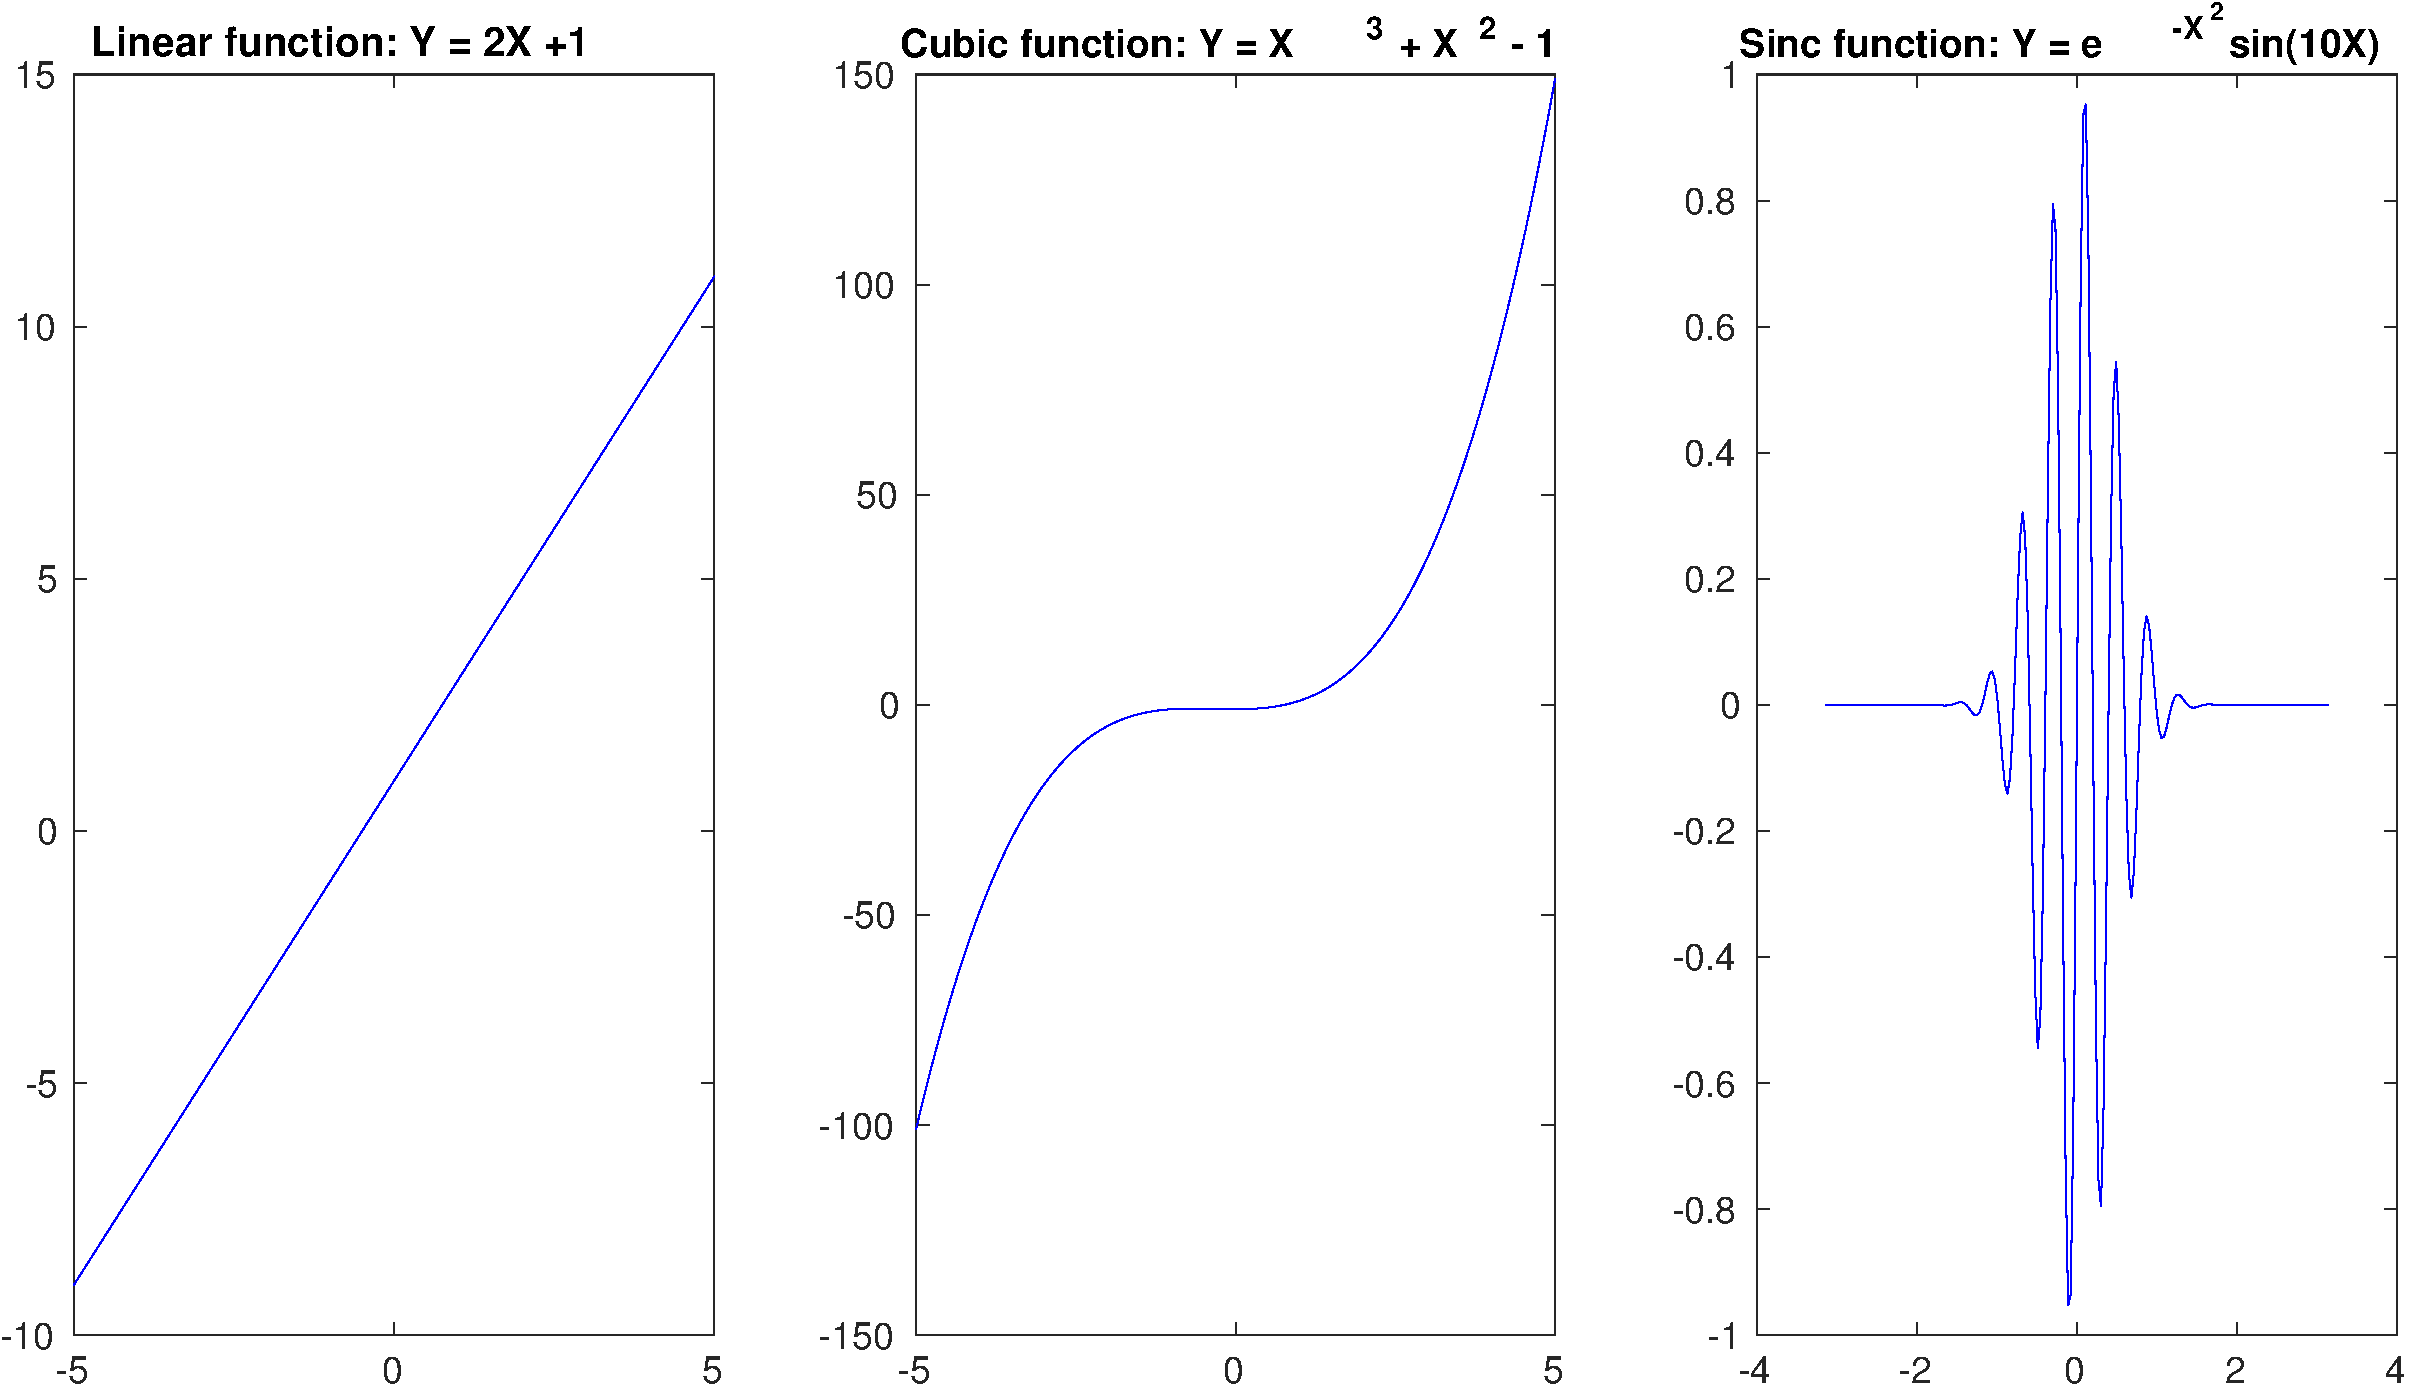
\includegraphics[scale=.30]{datasets.pdf}
    \caption{Functions to regress}
    \label{fig:regress_datasets}
\end{figure}

\subsection{Analysis}

I investigated the effect of fixing the amount of different settings
on the function estimation, here is their descriptions:

\begin{itemize}
\item $\epsilon$ or \emph{e} is the $\epsilon$-sensitive loss
  function;
\item $\sigma^2$ controls the bandwidth of the RBF kernel;
\item the polynomial kernel degree (1 means linear kernel);
\item $\gamma$ or \emph{bound} controls the amount of regularization
  (hence the smoothness of the decision boundary).
\end{itemize}

For the linear and cubic generated dataset, as expected I got good
results with polynomial kernel of degree 1 and 3 respectively. In
general, the RBF kernel worked well on all the dataset as they could
be tuned to fit well the data.

I did an extensive survey of the parameters for the first linear
dataset (see table \ref{table:dataset_lin}). On that particular set,
the linear kernel seem to have performed the best. Even for extremely
low $\epsilon$ (eg $\epsilon=0.005$), the number of support vectors
needed to describe the classifier is equal to two. Another obvious
advantage of that kernel was that no wiggle artefact appeared, in
contrast with the other more flexible kernels. Note that this
performance was achievable using the RBF kernel too, using a very
large $\sigma$ (as large values of that parameter tend to make
decision boundaries linear).

\begin{table}[H]
  \centering
  \begin{tabular}{l|r|r|r|r|r|r|r|r|r|r|}
    \cline{2-11}
    & \multicolumn{5}{l|}{e-value (Bound set to Inf)}                                                                                                 & \multicolumn{5}{l|}{Bound (e-value set to 0.1)}                                                                                           \\ \cline{2-11} 
    & \multicolumn{1}{l|}{0.005} & \multicolumn{1}{l|}{0.01} & \multicolumn{1}{l|}{0.05} & \multicolumn{1}{l|}{0.1} & \multicolumn{1}{l|}{0.5} & \multicolumn{1}{l|}{0.01} & \multicolumn{1}{l|}{0.1} & \multicolumn{1}{l|}{1} & \multicolumn{1}{l|}{10} & \multicolumn{1}{l|}{100} \\ \hline
    \multicolumn{1}{|l|}{Poly 1}             & 2                          & 2                         & 2                         & 2                        & 2                        & 20 **                     & 20 **                    & 13                     & 2                       & 100                      \\ \hline
    \multicolumn{1}{|l|}{Poly 2}             & 3                          & 6                         & 6                         & 6                        & 3                        & 20 **                     & 20 **                    & 8                      & 3                       & 3                        \\ \hline
    \multicolumn{1}{|l|}{Poly 3}             & 7                          & 7                         & 4                         & 4                        & 2 *                      & 20 **                     & 20 **                    & 15 *                   & 4 *                     & 4 *                      \\ \hline
    \multicolumn{1}{|l|}{Poly 4}             & 5                          & 5                         & 5                         & 5                        & 4 *                      & 20 **                     & 20 **                    & 14 *                   & 5 *                     & 5 *                      \\ \hline
    \multicolumn{1}{|l|}{RBF $\sigma^2=1$}   & 16                         & 7                         & 7                         & 4                        & 4 *                      & 20 **                     & 20 **                    & 20 **                  & 15 **                   & 4                        \\ \hline
    \multicolumn{1}{|l|}{RBF $\sigma^2=0.5$} & 10                         & 9                         & 9                         & 7                        & 5 *                      & 20 **                     & 20 **                    & 20 **                  & 10 **                   & 7 *                      \\ \hline
  \end{tabular}
  \caption{Number of support vectors required for different kernels and parameters (*: wiggle artefact visible, **: function estimation completely off)}
  \label{table:dataset_lin}
\end{table}

A general remark concerning the regularization applied via the bound
parameter, is that if too little of it is applied, the regression
performs poorly on my artificial datasets. Given that it controls how
error is allowed in the model, this makes sense. The same remark goes
for the e-value, which controls the loss function. If this value is
small, the model doesn't allow for a large margin.

The sparsity property is directly related to the kernel matrix of the
dual formulation of the SVM, in which the support vectors can be
found. Often that matrix will be sparse and fewer support vectors will
be needed than the number of datapoints n. The kernel matrix is
n-by-n, hence potentially, you could have situations where n support
vectors are needed, a very ``not'' sparse situation. 

The SVM regression formulated in the dual model using the lagrangians
is akin to non-parametric modelling. In that sense, it is very
different from least-squares fit.

\newpage
\section{Sum of Cosines}

I started by investigating the regression of the function with a given
$\sigma^2$ value of 0.1. The results are visually reported on figure
\ref{fig:sumcos1}, and were produced by the following code:

\begin{lstlisting}
gam_list = [1000, 100, 10, 1];
sig2_list = [0.1, 0.1, 0.1, 0.1];
figure('Color',[1 1 1]);

for i = 1:4
    gam = gam_list(i); sig2 = sig2_list(i);
    [alpha, b] = trainlssvm({Xtrain, Ytrain, 'f', gam, sig2, 'RBF_kernel'});
    YtestEst = simlssvm({Xtrain, Ytrain, 'f', gam, sig2, 'RBF_kernel'},{alpha, b}, Xtest);
    subplot(2,2,i);
    plot(XX, YY, 'k-'); hold on; 
    plot(Xtest, Ytest, '.'); hold on; 
    plot(Xtest, YtestEst, 'r+');
    legend('true', 'Ytest', 'YtestEst');
end
\end{lstlisting}

\begin{figure}[H]
    \centering
    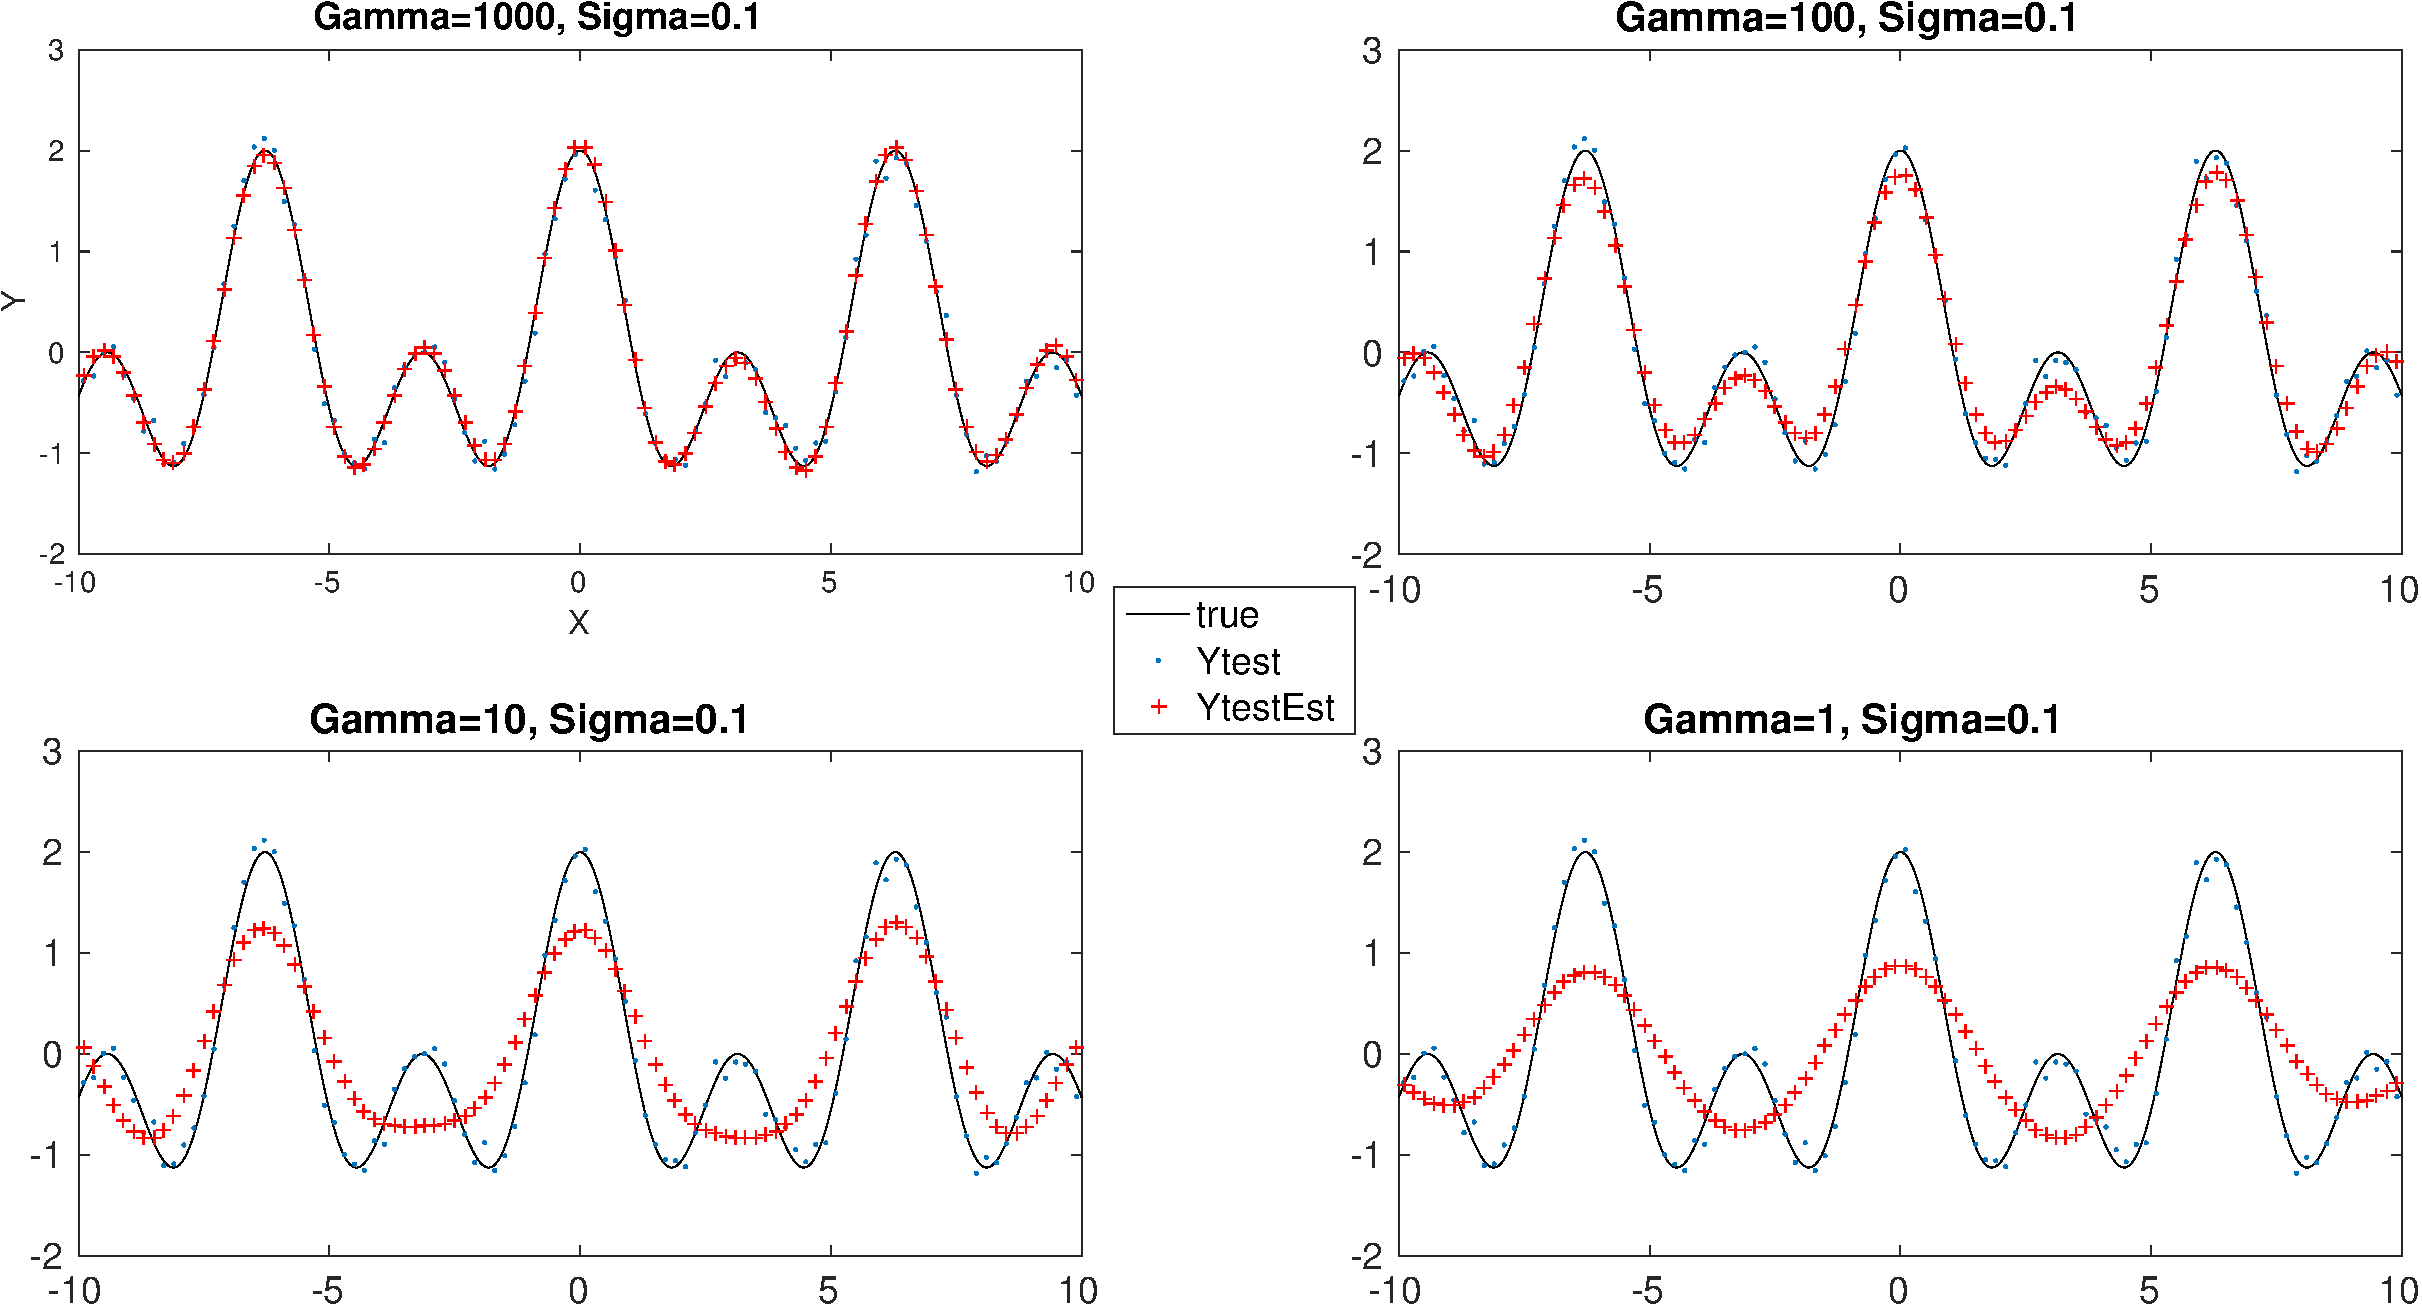
\includegraphics[scale=.40]{sumcos1.pdf}
    \caption{Function estimation for various values of $\gamma$ (fixed
      $\sigma^2$)}
    \label{fig:sumcos1}
\end{figure}

I then investigated the function estimation for a fixed value of
$\gamma$ using similar code. The visual results can be seen on figure
\ref{fig:sumcos2}

\begin{figure}[H]
  \vspace{-50pt}
    \centering
    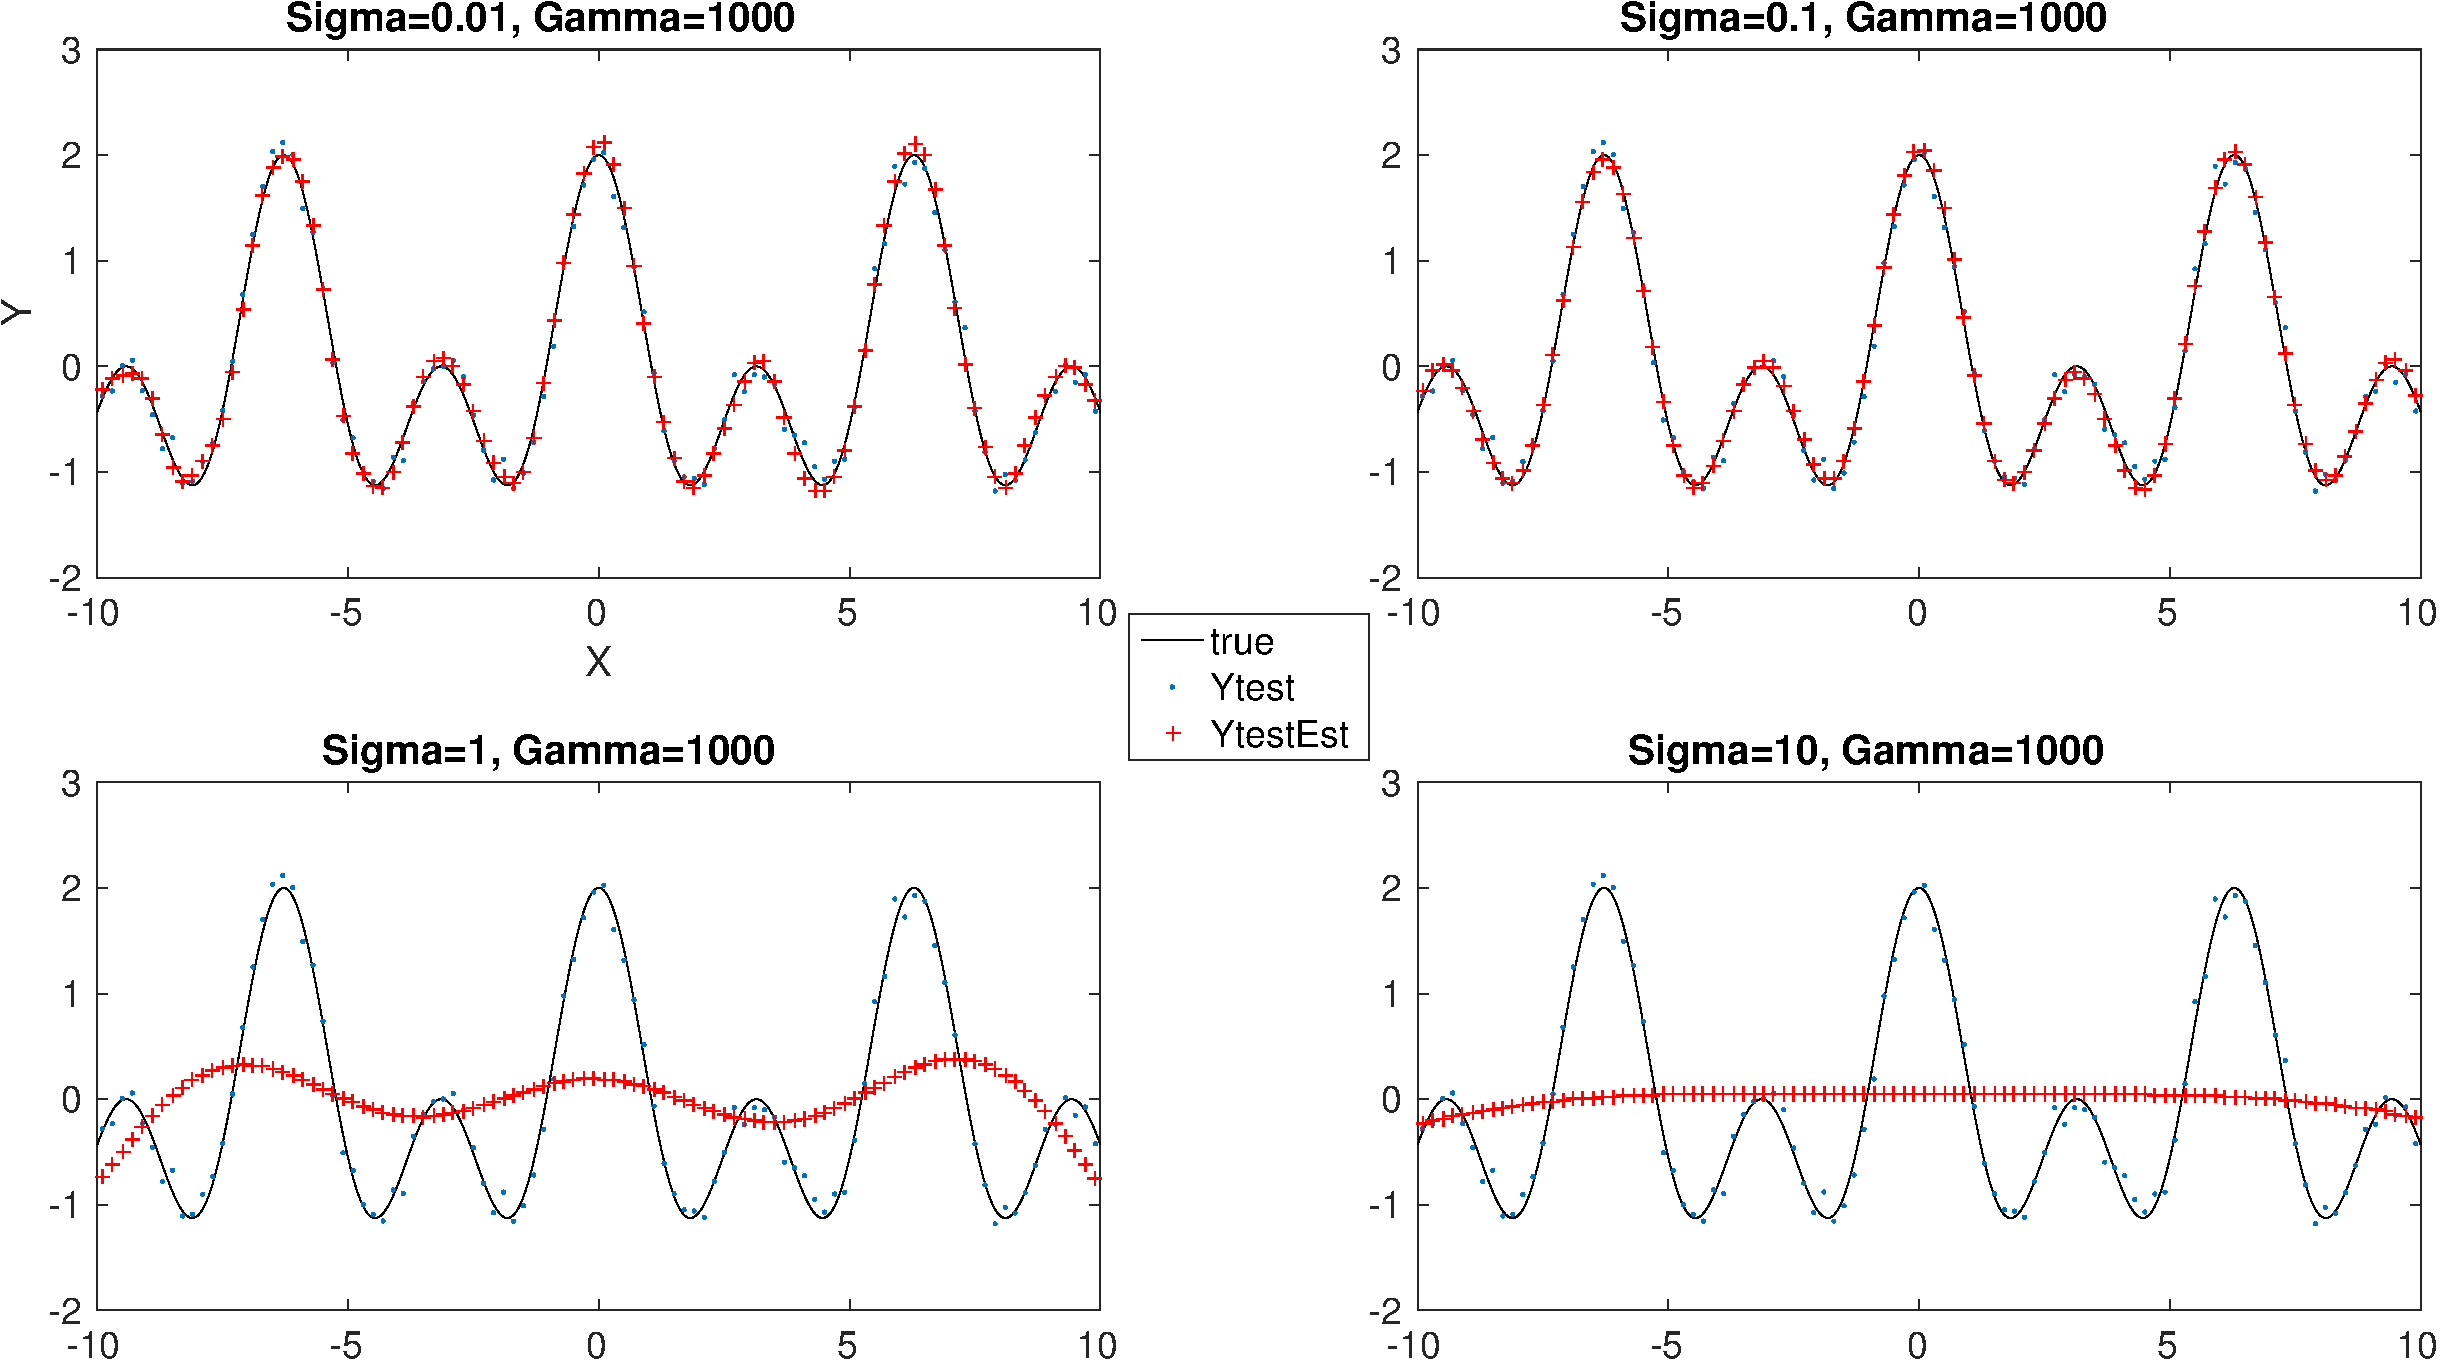
\includegraphics[scale=.40]{sumcos2.pdf}
    \caption{Function estimation for various values of $\sigma^2$ (fixed
      $\gamma$)}
    \label{fig:sumcos2}
\end{figure}

One of the question from this exercise is to determine whether there
is an optimal pair of parameters that would reach the best
estimation. Although the SVM formulation is convex, and thus has a
single solution, when we start exploring hyperparameter space, the
problem is no more convex. 

As such, I thought that there would not be a single pair, and decided
to verify this by computing and visualizing the error surface
consisting of systematic evaluation between the estimated Y for a
given pair of $\sigma^2$ and $\gamma$ and the true Y (known in our
case given that we are working with a synthetic dataset.) Here is the
code I used for this part:

\begin{lstlisting}
gam_list = logspace(-2,2,100); sig2_list = logspace(-2,1,100);
err_matrix = zeros(100,100); i = 1; j = 1;
true_ys = cos(Xtest) + cos(2.*Xtest);

for sig2=sig2_list,
    j = 1;
    for gam=gam_list,
        [alpha, b] = trainlssvm({Xtrain, Ytrain, 'f', gam, sig2, 'RBF_kernel'});
        YtestEst = simlssvm({Xtrain, Ytrain, 'f', gam, sig2, 'RBF_kernel'},{alpha, b}, Xtest);
        err_matrix(i, j) = sum((YtestEst - true_ys).^2);
        j = j + 1;
    end
    i = i + 1;
end

figure('Color',[1,1,1]);
h = surf(gam_list, sig2_list, err_matrix);
set(get(h,'Parent'),'XScale','log');
set(get(h,'Parent'),'YScale','log');
\end{lstlisting}

The result of the parameter space exploration can be seen on figure
\ref{fig:sumcos_surf}. One can recognize that there is indeed no
single best pair of parameters to obtain. In general a large gamma
will reap better results in lowering the error for this synthetic
dataset. It also seem that for larger $\gamma$, the value of
$\sigma^2$ can be increased too.

\begin{figure}[H]
  \vspace{-60pt}
    \centering
    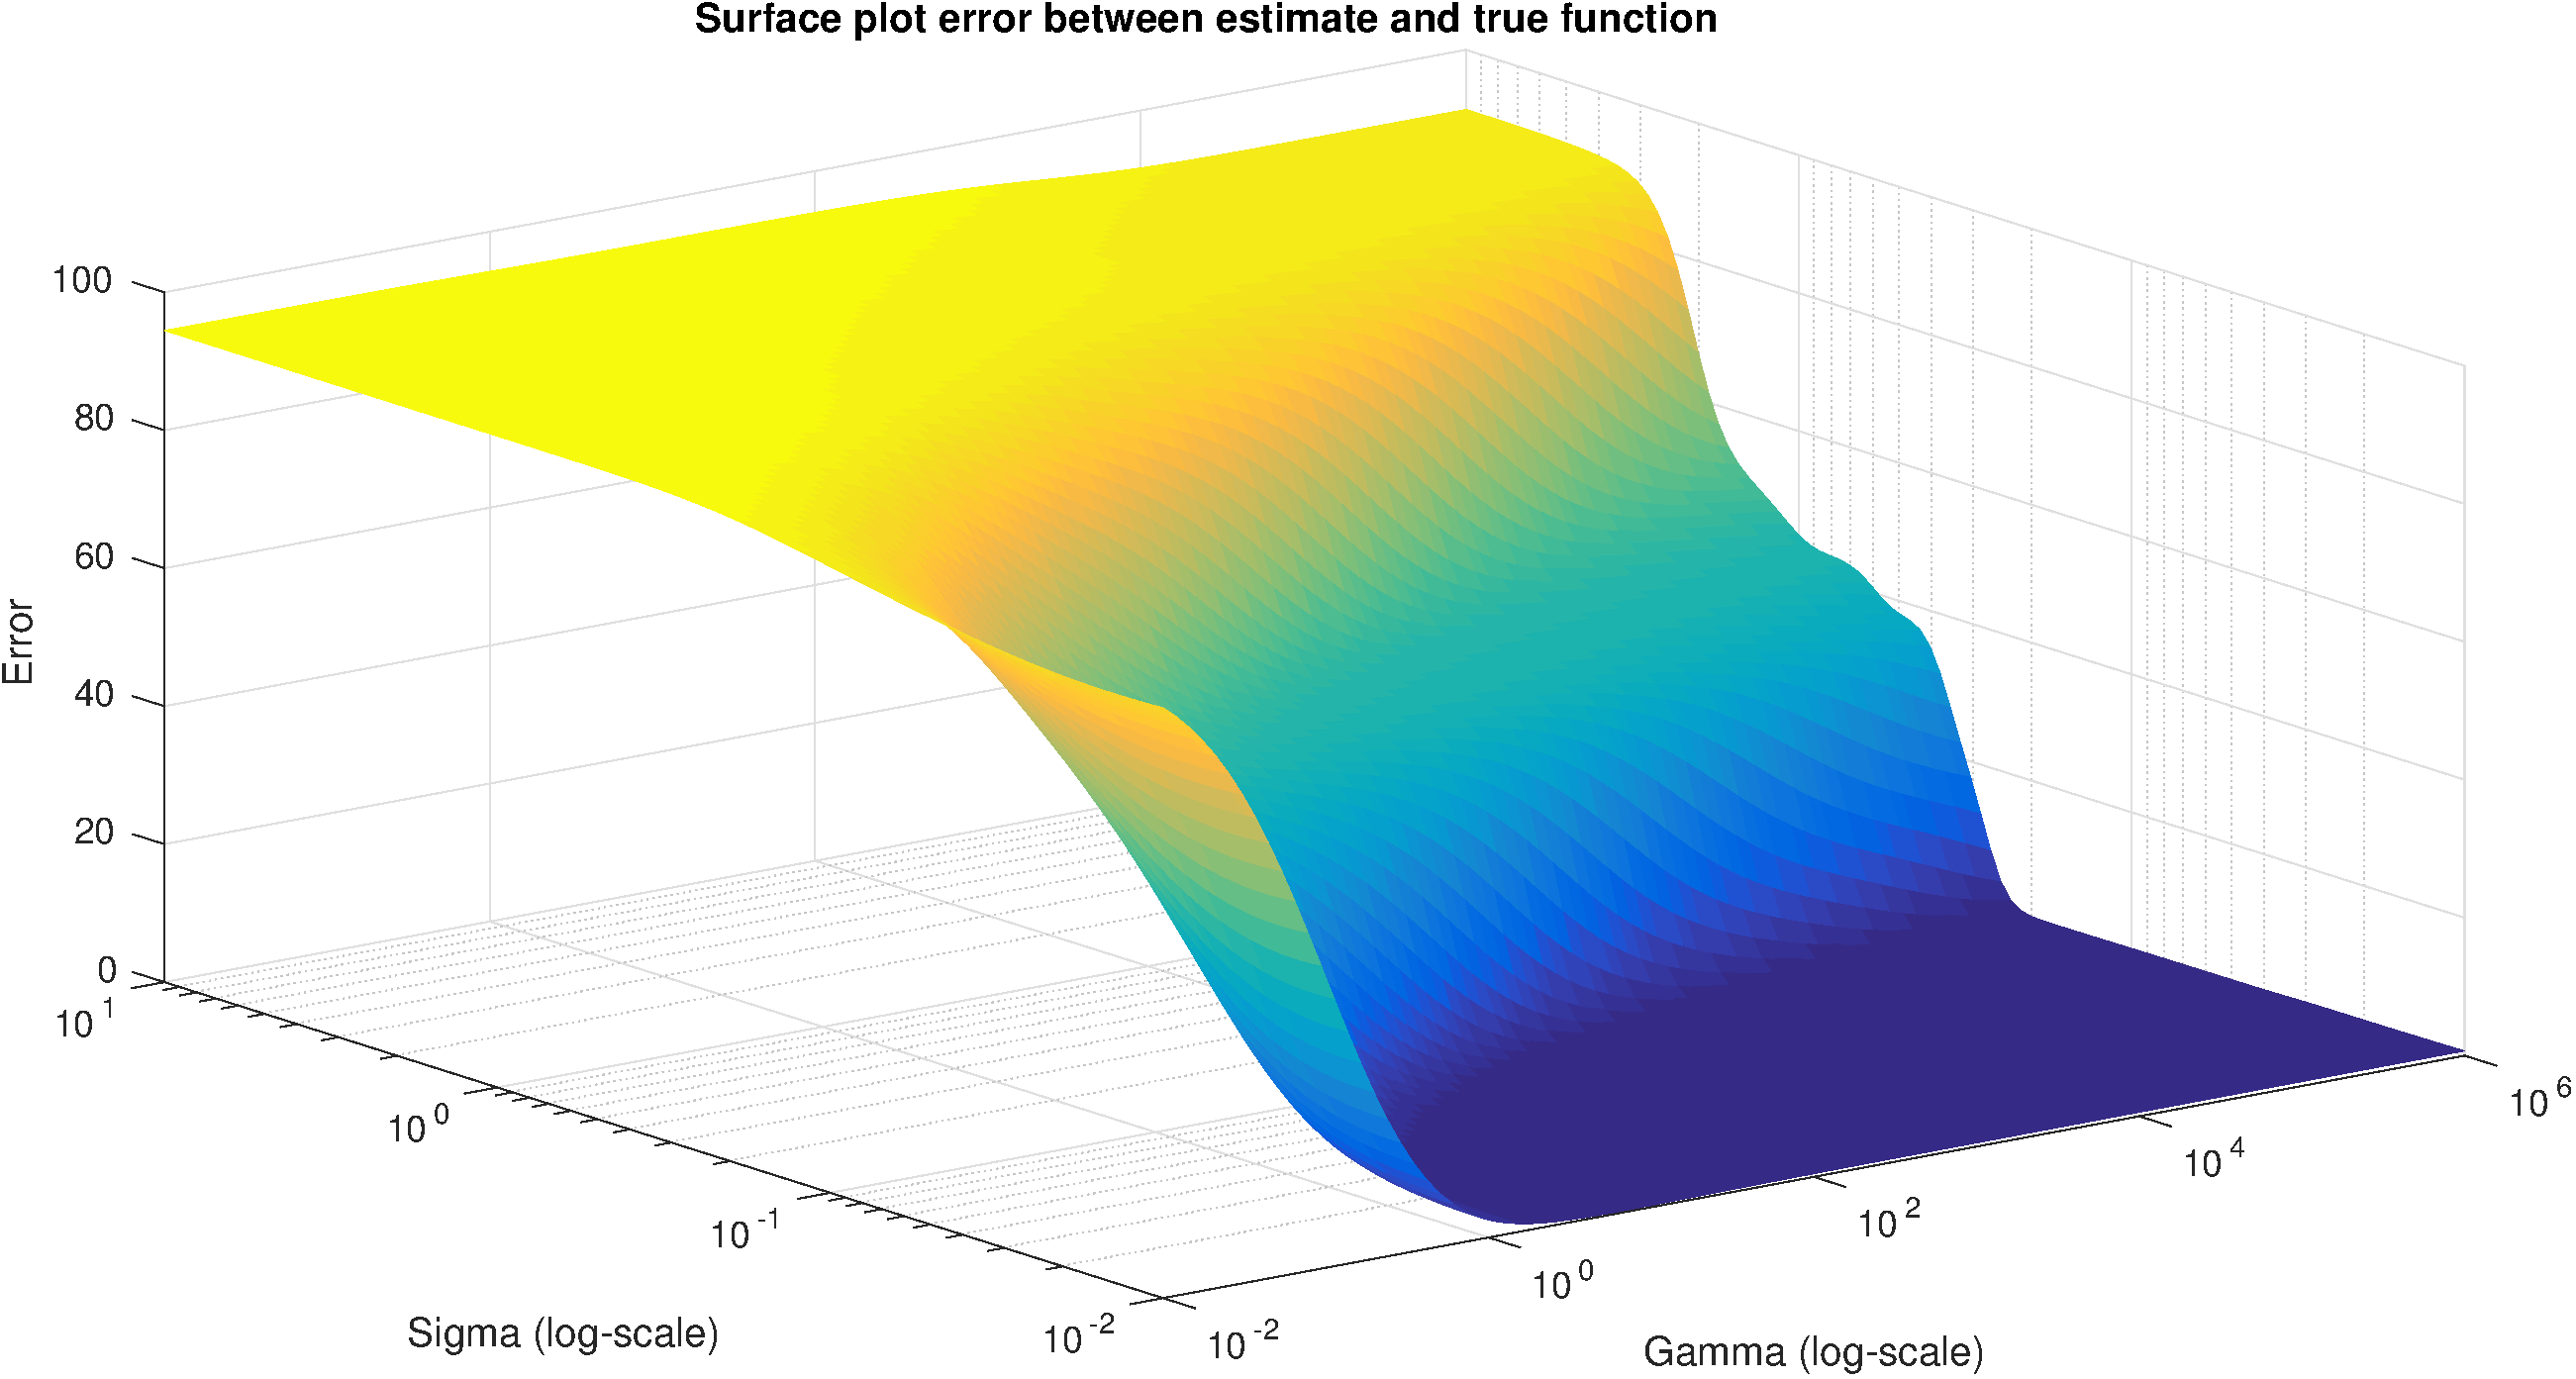
\includegraphics[scale=.40]{sumcos_surf.pdf}
    \caption{Exploration of parameter space effect on the function estimation}
    \label{fig:sumcos_surf}
\end{figure}



\section{Hyper-parameter Tuning}

In order to tune the parameters, I used a combination of the 2 global
optimisation techniques available (coupled-simulated annealing and
randomized directional search) with the 2 techniques to select the
values of the hyperparameters (simplex and gridsearch). I could not
see any difference in the result of the function estimation. All the
values returned were systematically in the area of low test error
discovered in the previous section.

\begin{figure}[H]
    \centering
    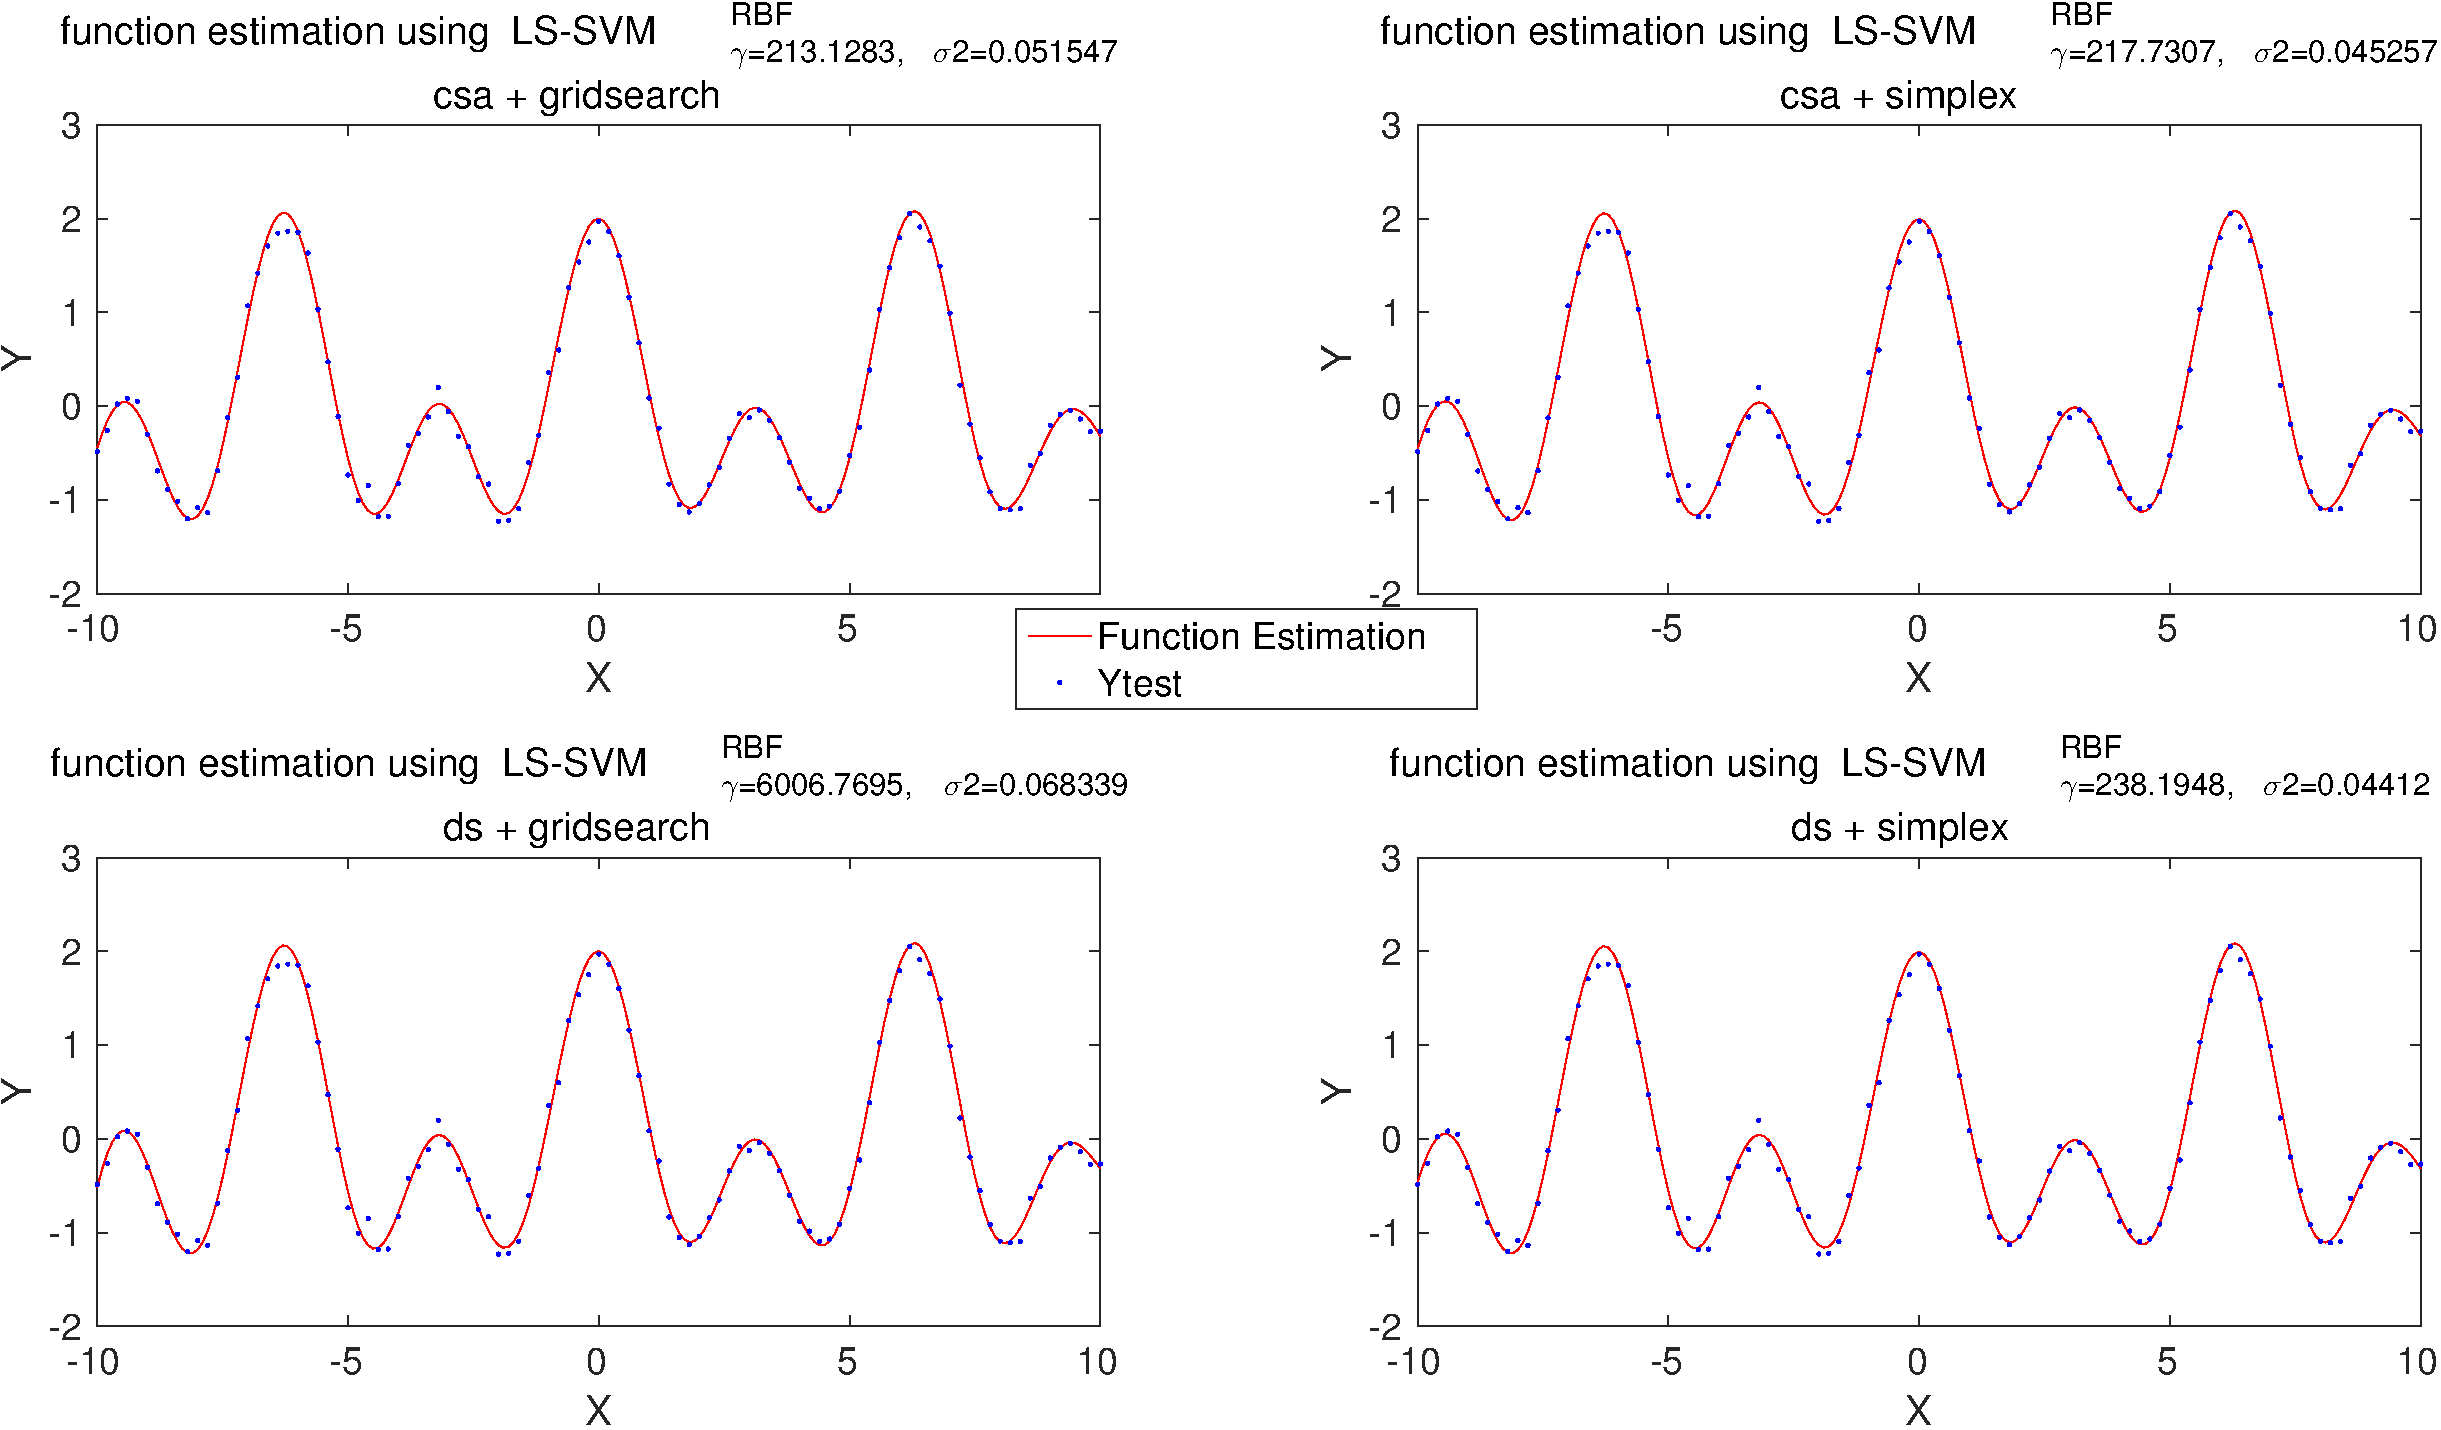
\includegraphics[scale=.40]{hyperparam_tuning.pdf}
    \caption{Parameter tuning with heuristics}
    \label{fig:hyperparam_tuning}
\end{figure}

The speed of execution can be estimated using the tic/toc commands in
matlab. The results in execution time in seconds are reported in table
\ref{tab:computing_param}. It would seem on this small experiment,
that the csa+simplex technique is faster at converging in the search
space of $\gamma$ and $\sigma^2$ than ds+gridsearch.

As mentioned in the previous assignment, although the formulation of
the SVM problem is indeed convex, we are faced here with a problem of
hyperparameter selection, which is non-convex, and multiple local
minima are thus possible. 

The technique \emph{csa} and \emph{ds} are global optimization
techniques that can help with the search (though without garantees of
locating a global minimum). In a first step, those techniques will act
to select in the landscape a place to start the search, which is then
finalized using a \emph{simplex} approach, or a pre-defined
\emph{searchgrid}. This explains the significant variability in the
returned \emph{optimized} parameters, and in the speed of
convergence. Whereas \emph{gridsearch} locates a minimum using a grid
of parameter values, \emph{simplex} finds a minimum from a given
starting value by different types of movement (so-called
reflection/expansion/contraction). Hence the search is faster (though
less exhaustive) using \emph{simplex}

\begin{table}[H]
  \centering
  \begin{tabular}{l|l|l|l|l|l|l|}
    \cline{2-7}
    & run 1 & run 2 & run 3 & run 4 & run 5 & avg  \\ \hline
    \multicolumn{1}{|l|}{csa + simplex}    & 0.59  & 0.68  & 0.66  & 0.66  & 0.61  & 0.64 \\ \hline
    \multicolumn{1}{|l|}{csa + gridsearch} & 1.01  & 0.92  & 0.95  & 0.92  & 0.91  & 0.94 \\ \hline
    \multicolumn{1}{|l|}{ds + simplex}     & 0.96  & 0.72  & 0.64  & 0.79  & 0.60  & 0.74 \\ \hline
    \multicolumn{1}{|l|}{ds + gridsearch}  & 1.06  & 1.11  & 1.29  & 1.07  & 1.08  & 1.12 \\ \hline
  \end{tabular}
  \caption{Computing time (seconds)}
  \label{tab:computing_param}
\end{table}

% \begin{figure}[H]
%     \centering
%     \begin{subfigure}{.5\textwidth}
%       \centering
%       \includegraphics[width=0.9\linewidth]{1-2-1-kernel7.png}
%       \caption{Support vectors reduce dataset}
%       \label{fig:ker7reduced}
%     \end{subfigure}%
%     \begin{subfigure}{.5\textwidth}
%       \centering
%       \includegraphics[width=0.9\linewidth]{1-2-1-kernel7spiral.png}
%       \caption{No compression}
%       \label{fig:ker7spiral}
%     \end{subfigure}
%     \caption{Support vectors}
%     \label{fig:ker7}
% \end{figure}

\section{Application of the Bayesian framework}

In this section, we investigate the use of the bayes rule for the
tuning and analysis of function approximation (with a quick incursion
in the classification task). Originally introduced within the context
of VC-theory, support vector machines have little to do with a
probabilistic point of view. The introduction of kernel functions such
as RBF however create a link with that world.

An interesting contribution of the introduction of such a
probabilistic setting is related to the inference of the parameters,
critical to building a coherent SVM model. As seen before, one way to
deal with their estimation is via the use of a validation set. Here,
we will see that the parameters can be deduced through the application
of the Bayes rule within a hierarchical model without the use of a
validation set. We will work with a RBF kernel function, and thus we
will have 3 levels of inference.

Using the same dataset as previously (sum of cosines), we can build
our model using the \emph{bay\_optimize} function. Note that the
examples in the assignment work on the training set, but there is no
real need to limit them. 

\begin{lstlisting}
[~,alpha,b] = bay_optimize({X,Y,'f',gam,sig2}, 1);
[~,gam] = bay_optimize({X,Y,'f',gam,sig2},2);
[~,sig2] = bay_optimize({X,Y,'f',gam,sig2},3);
sig2e = bay_errorbar({X,Y,'f',gam,sig2},'figure');
\end{lstlisting}

The last line of code produces the figure \ref{fig:sumcos_bay1} on
which it is possible to visualize at least 2 key things. Firstly, that
the function estimation performed indeed very well, and secondly, that
it is possible to estimate the confidence interval of our regression.

\begin{figure}[H]
  \vspace{-20pt}
    \centering
    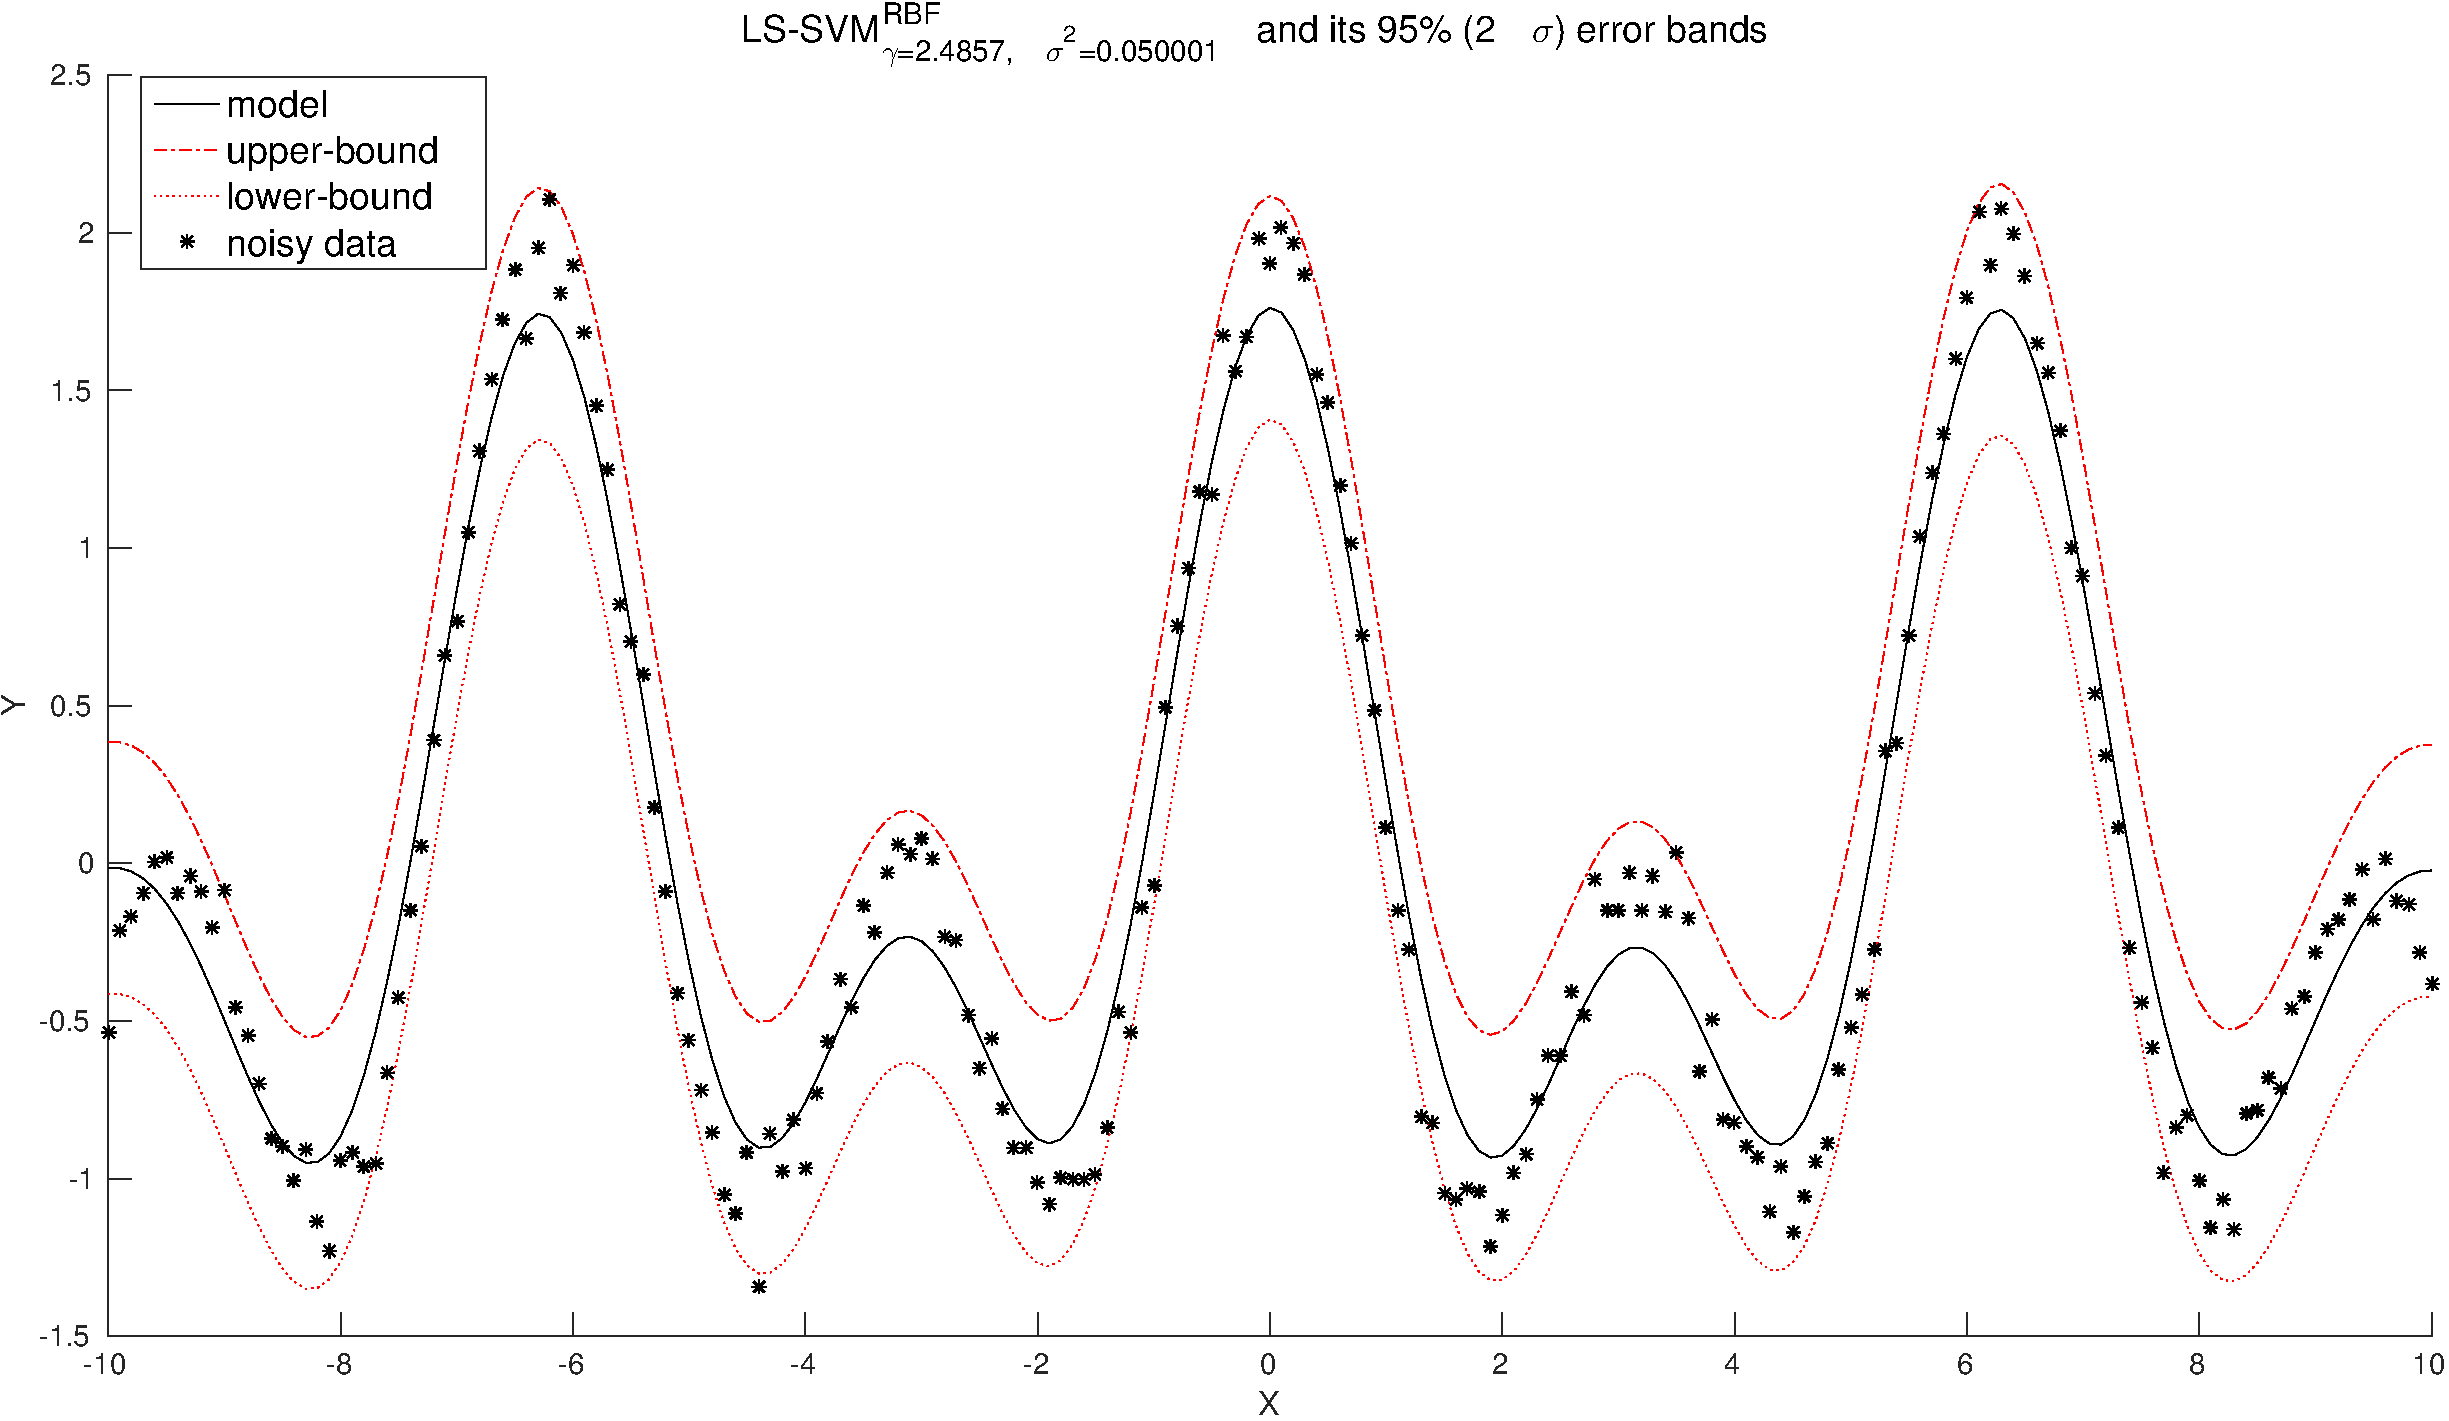
\includegraphics[scale=.40]{sumcos_bay1.pdf}
    \caption{Bayesian parameter estimation and resulting model with error bars}
    \label{fig:sumcos_bay1}
\end{figure}

A good way to visualize the dependence between the three levels of
inference of our model is to realize the connection that each level
has with the next one. Indeed, the so-called evidence bit of the bayes
rule of level 1 corresponds to the likelihood bit of level 2, whose
evidence is itself the likelihood of level 3. As illustrated
\footnote{J.Suykens, Support Vector Machines: Methods and Applications
chapter 4. Fig 4.1}:

\begin{figure}[H]
    \centering
    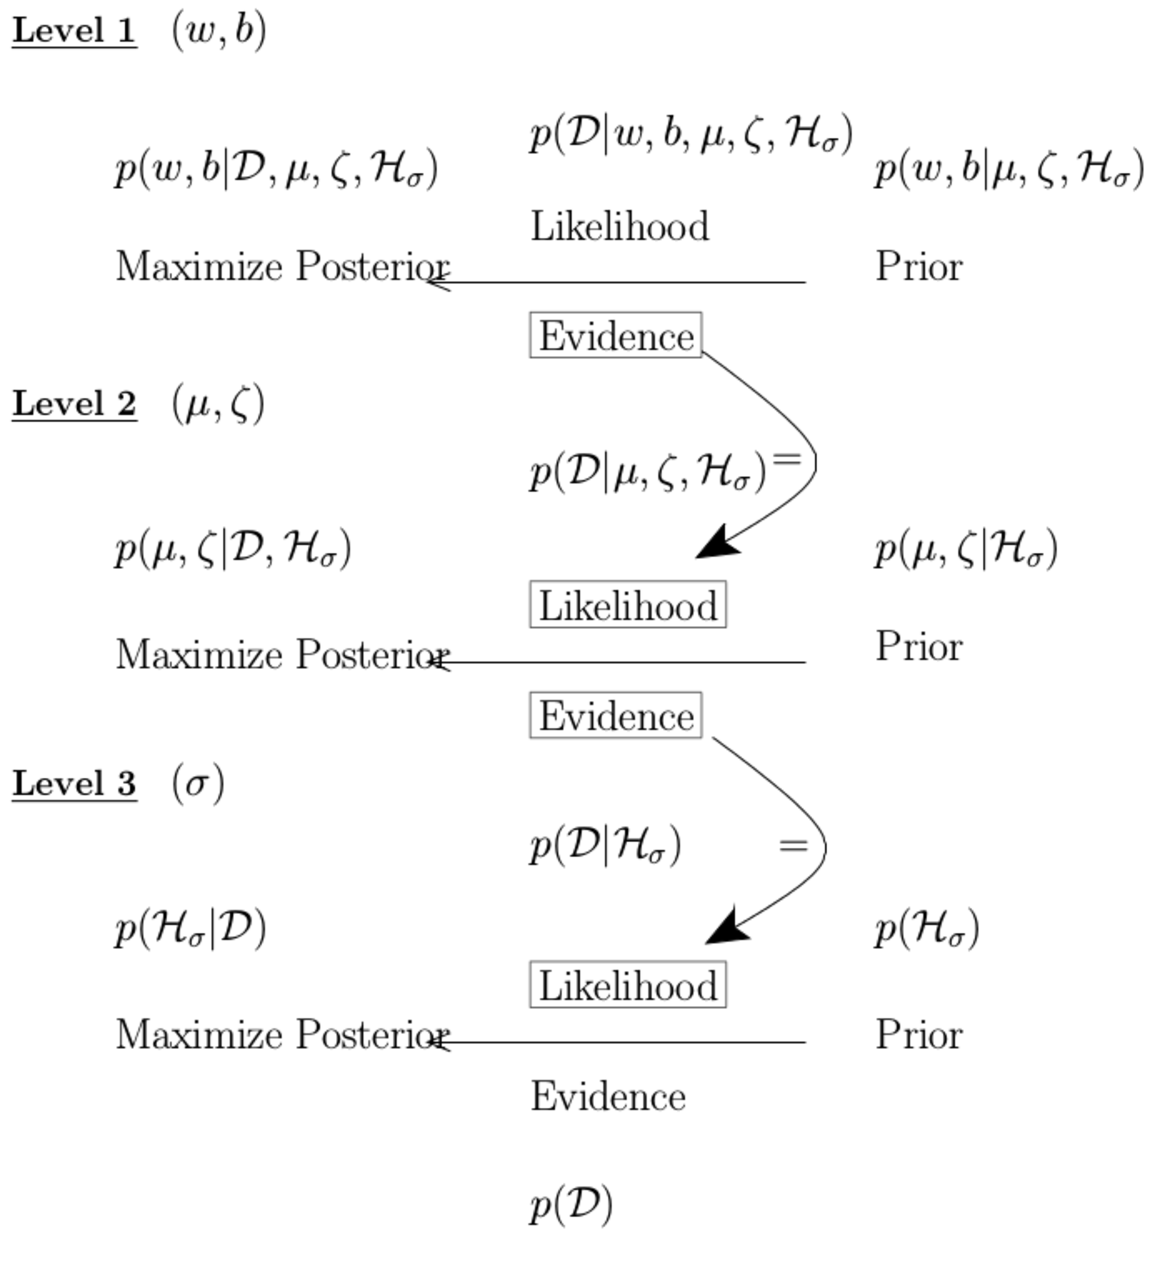
\includegraphics[scale=.46]{3level_bayesian.pdf}
    \label{fig:3level_bay1}
\end{figure}


The next figure \ref{fig:bayes_iris} reports the results from the
classification of the iris dataset. For this, the function
\emph{bay\_modoutClass} was used with an array of different
$\gamma \in \{1,10,100\}$ and $\sigma^2 \in \{0.01,0.1, 1\}$. The
colors can be interpreted as the probabilities of belonging to a given
class.

\begin{figure}[H]
    \centering
    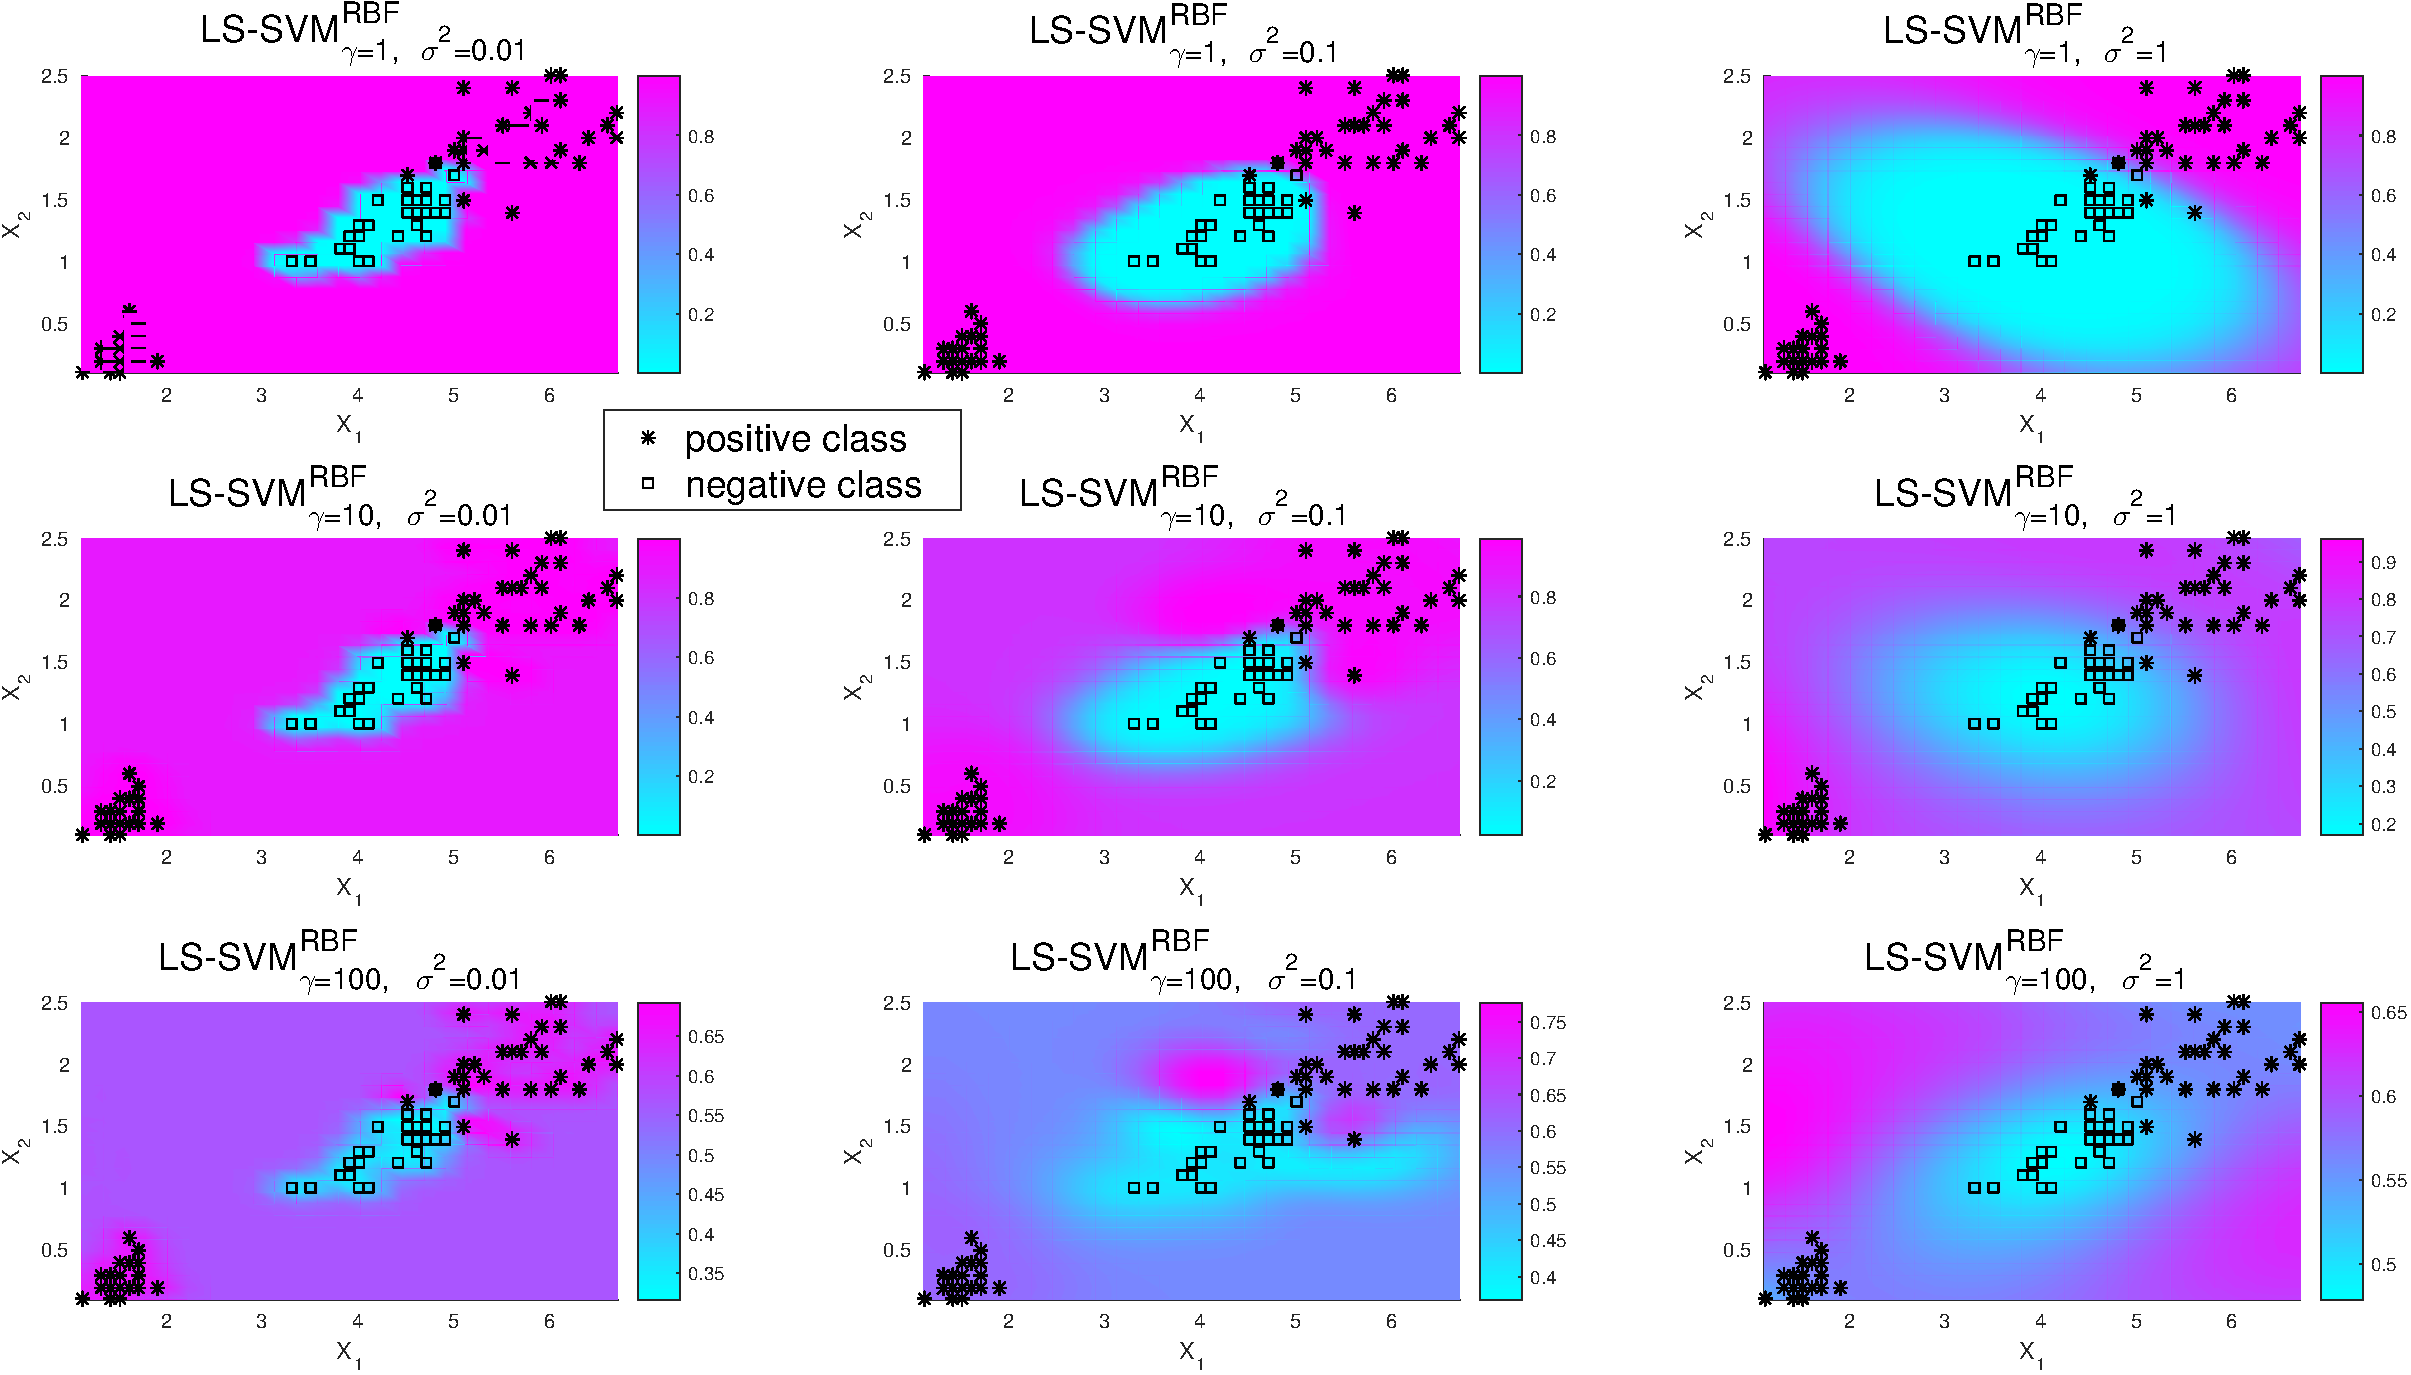
\includegraphics[scale=.40]{bayes_iris.pdf}
    \caption{Bayesian parameter estimation and resulting model with error bars}
    \label{fig:bayes_iris}
\end{figure}

The bayesian framework also enables the selection of the most relevant
inputs by automatic relevance determination (ARD). For this toy
dataset, it is possible to obtain it as such:

\begin{lstlisting}
X = 10.*rand(100,3)-3;
Y = cos(X(:,1)) + cos(2*(X(:,1))) + 0.3.*randn(100,1);
[selected, ranking] = bay_lssvmARD({X,Y,'class',gam,sig2});

>> ans =
SELECTED INPUT(S) ('discrete'): [1]
\end{lstlisting}

It should be possible to determine the best selection of inputs
similarly by doing crossvalidation using models with all combinations
of variables and estimate the test MSE. Note however that this is not
scalable as the combination explodes with the number of variables
O($2^p$). There may be a way to do something similar to variable
selection found in linear models (forward/backward selection).

\section{Robust regression}

Robust regression is an important set of techniques to deal with noisy
data that contains outliers. The figure \ref{fig:robust_ouliers} shows
what can happen when outliers are introduced. On the left-hand side,
we have a model that performs reasonably well at function
estimation. On the right-hand side, the same dataset has been
perturbed by the introduction of 6 outliers, and important shifts in
the function estimation ensue. The LS-SVM framework comes with a serie
of robust weighting function that can deal with outliers, as shown on
figure \ref{fig:bayes_robust}. As can be observed from the figure, all
methods return very similar function estimation.

\begin{figure}[H]
    \centering
    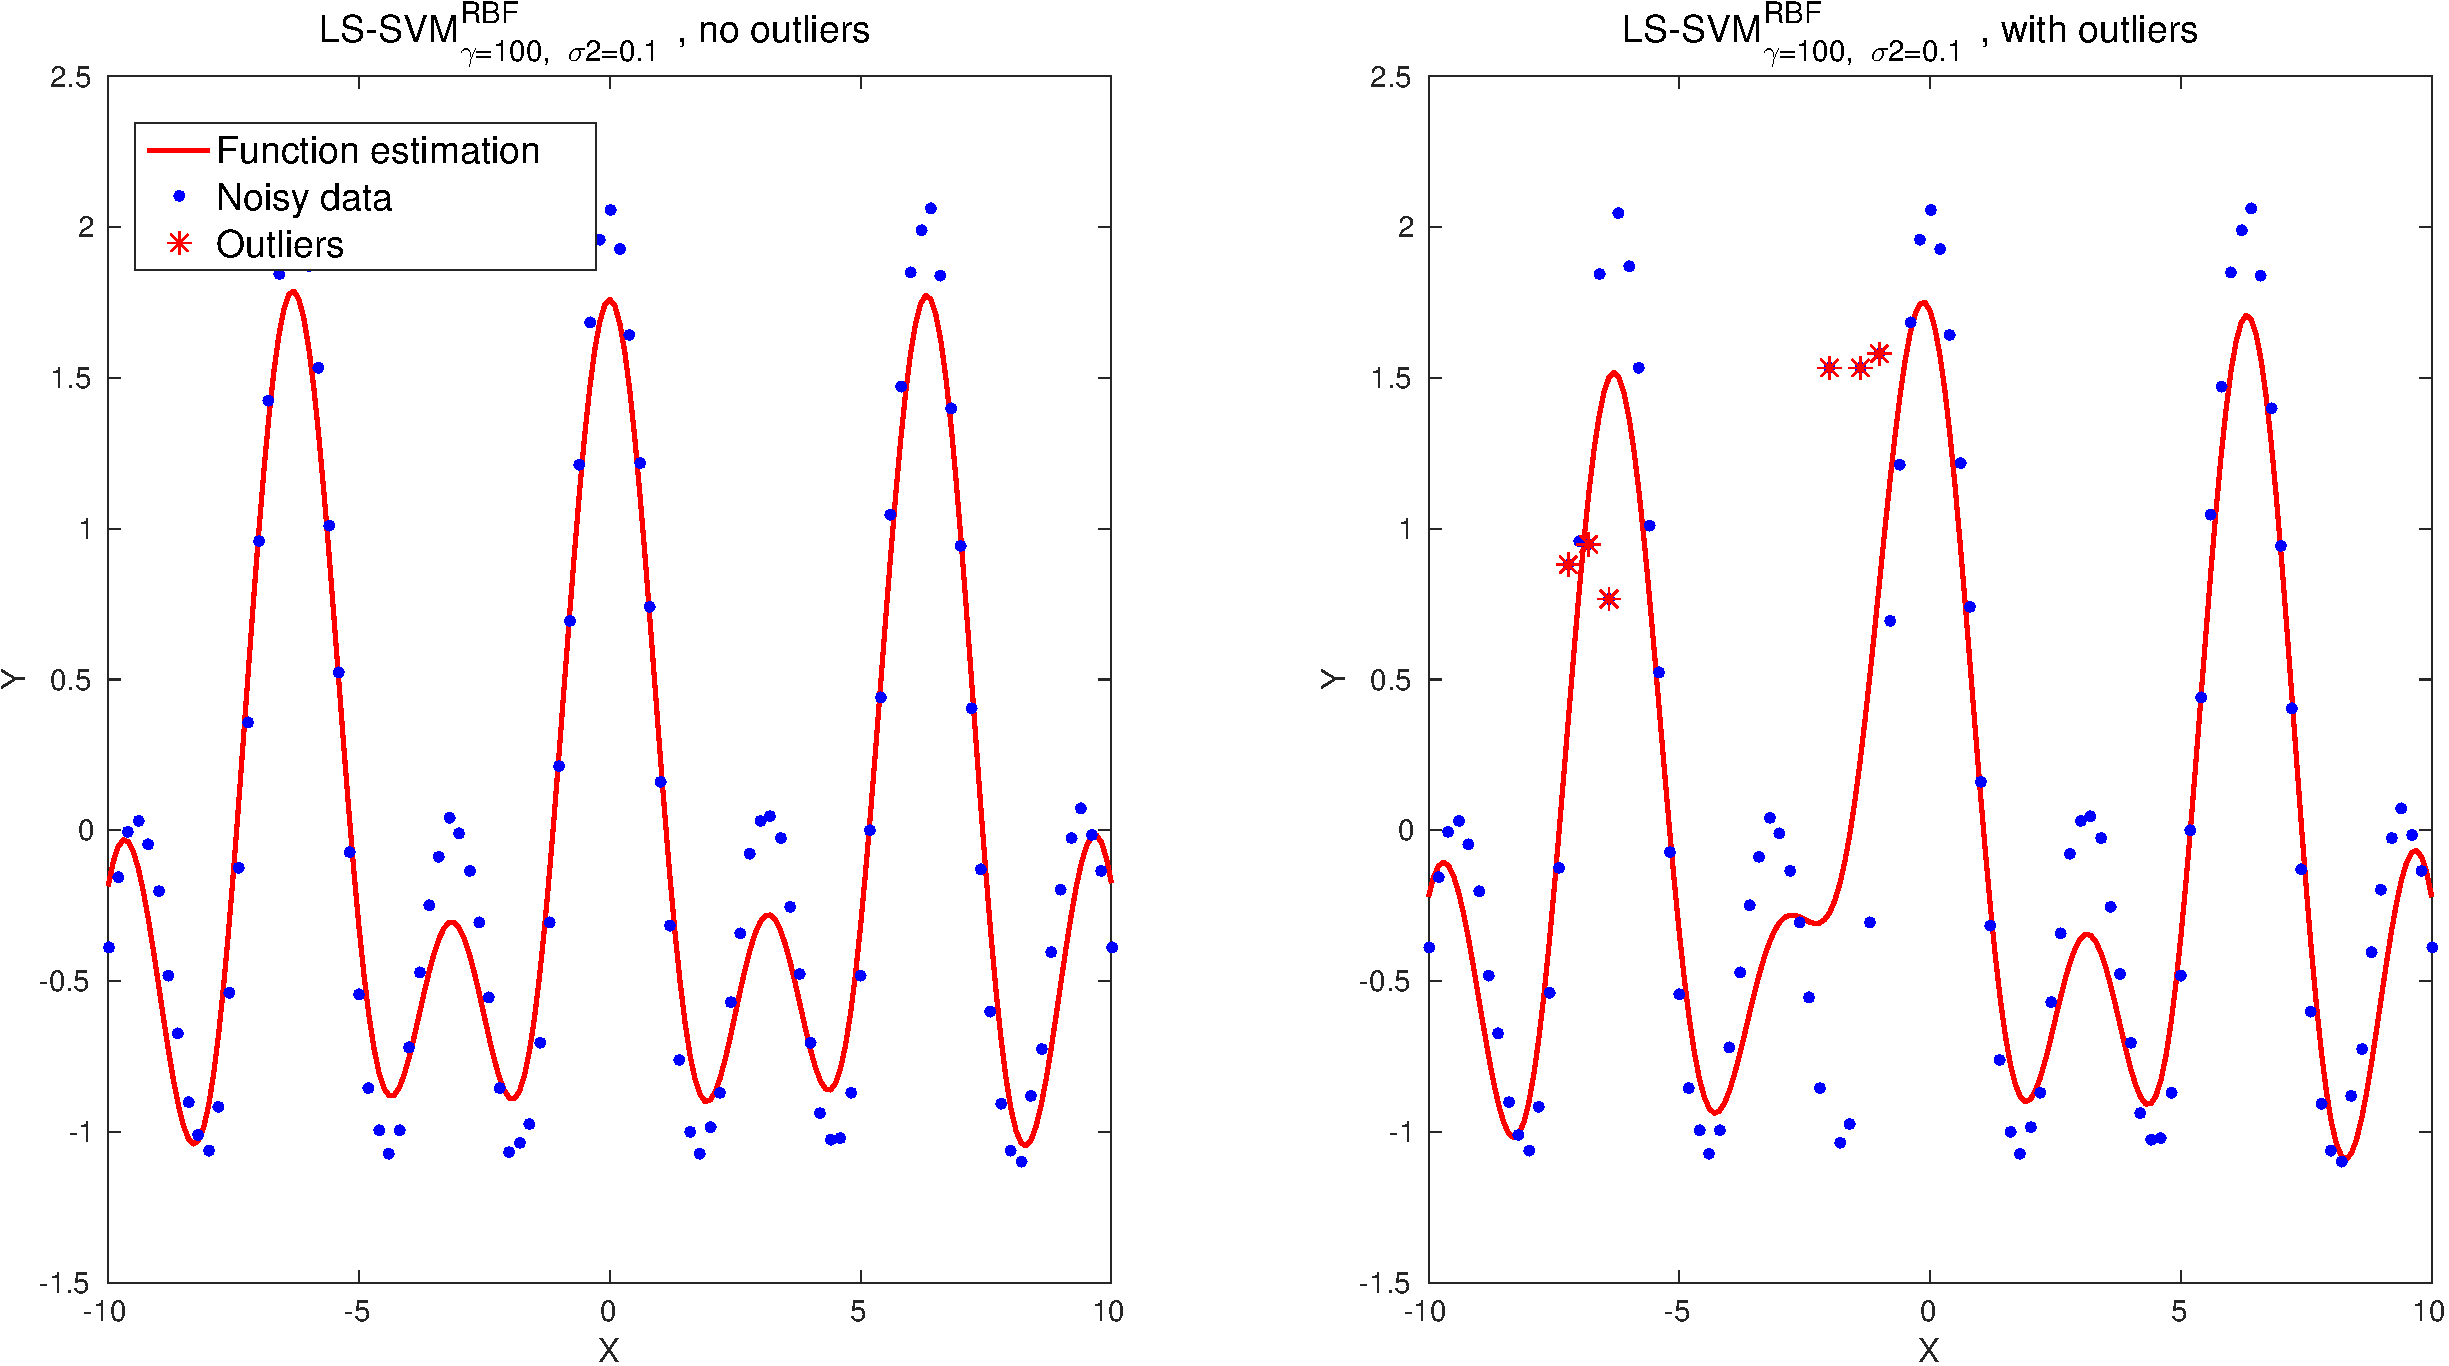
\includegraphics[scale=.40]{robust_outliers.pdf}
    \caption{Robust vs. non-robust model}
    \label{fig:robust_ouliers}
\end{figure}

\begin{figure}[H]
    \centering
    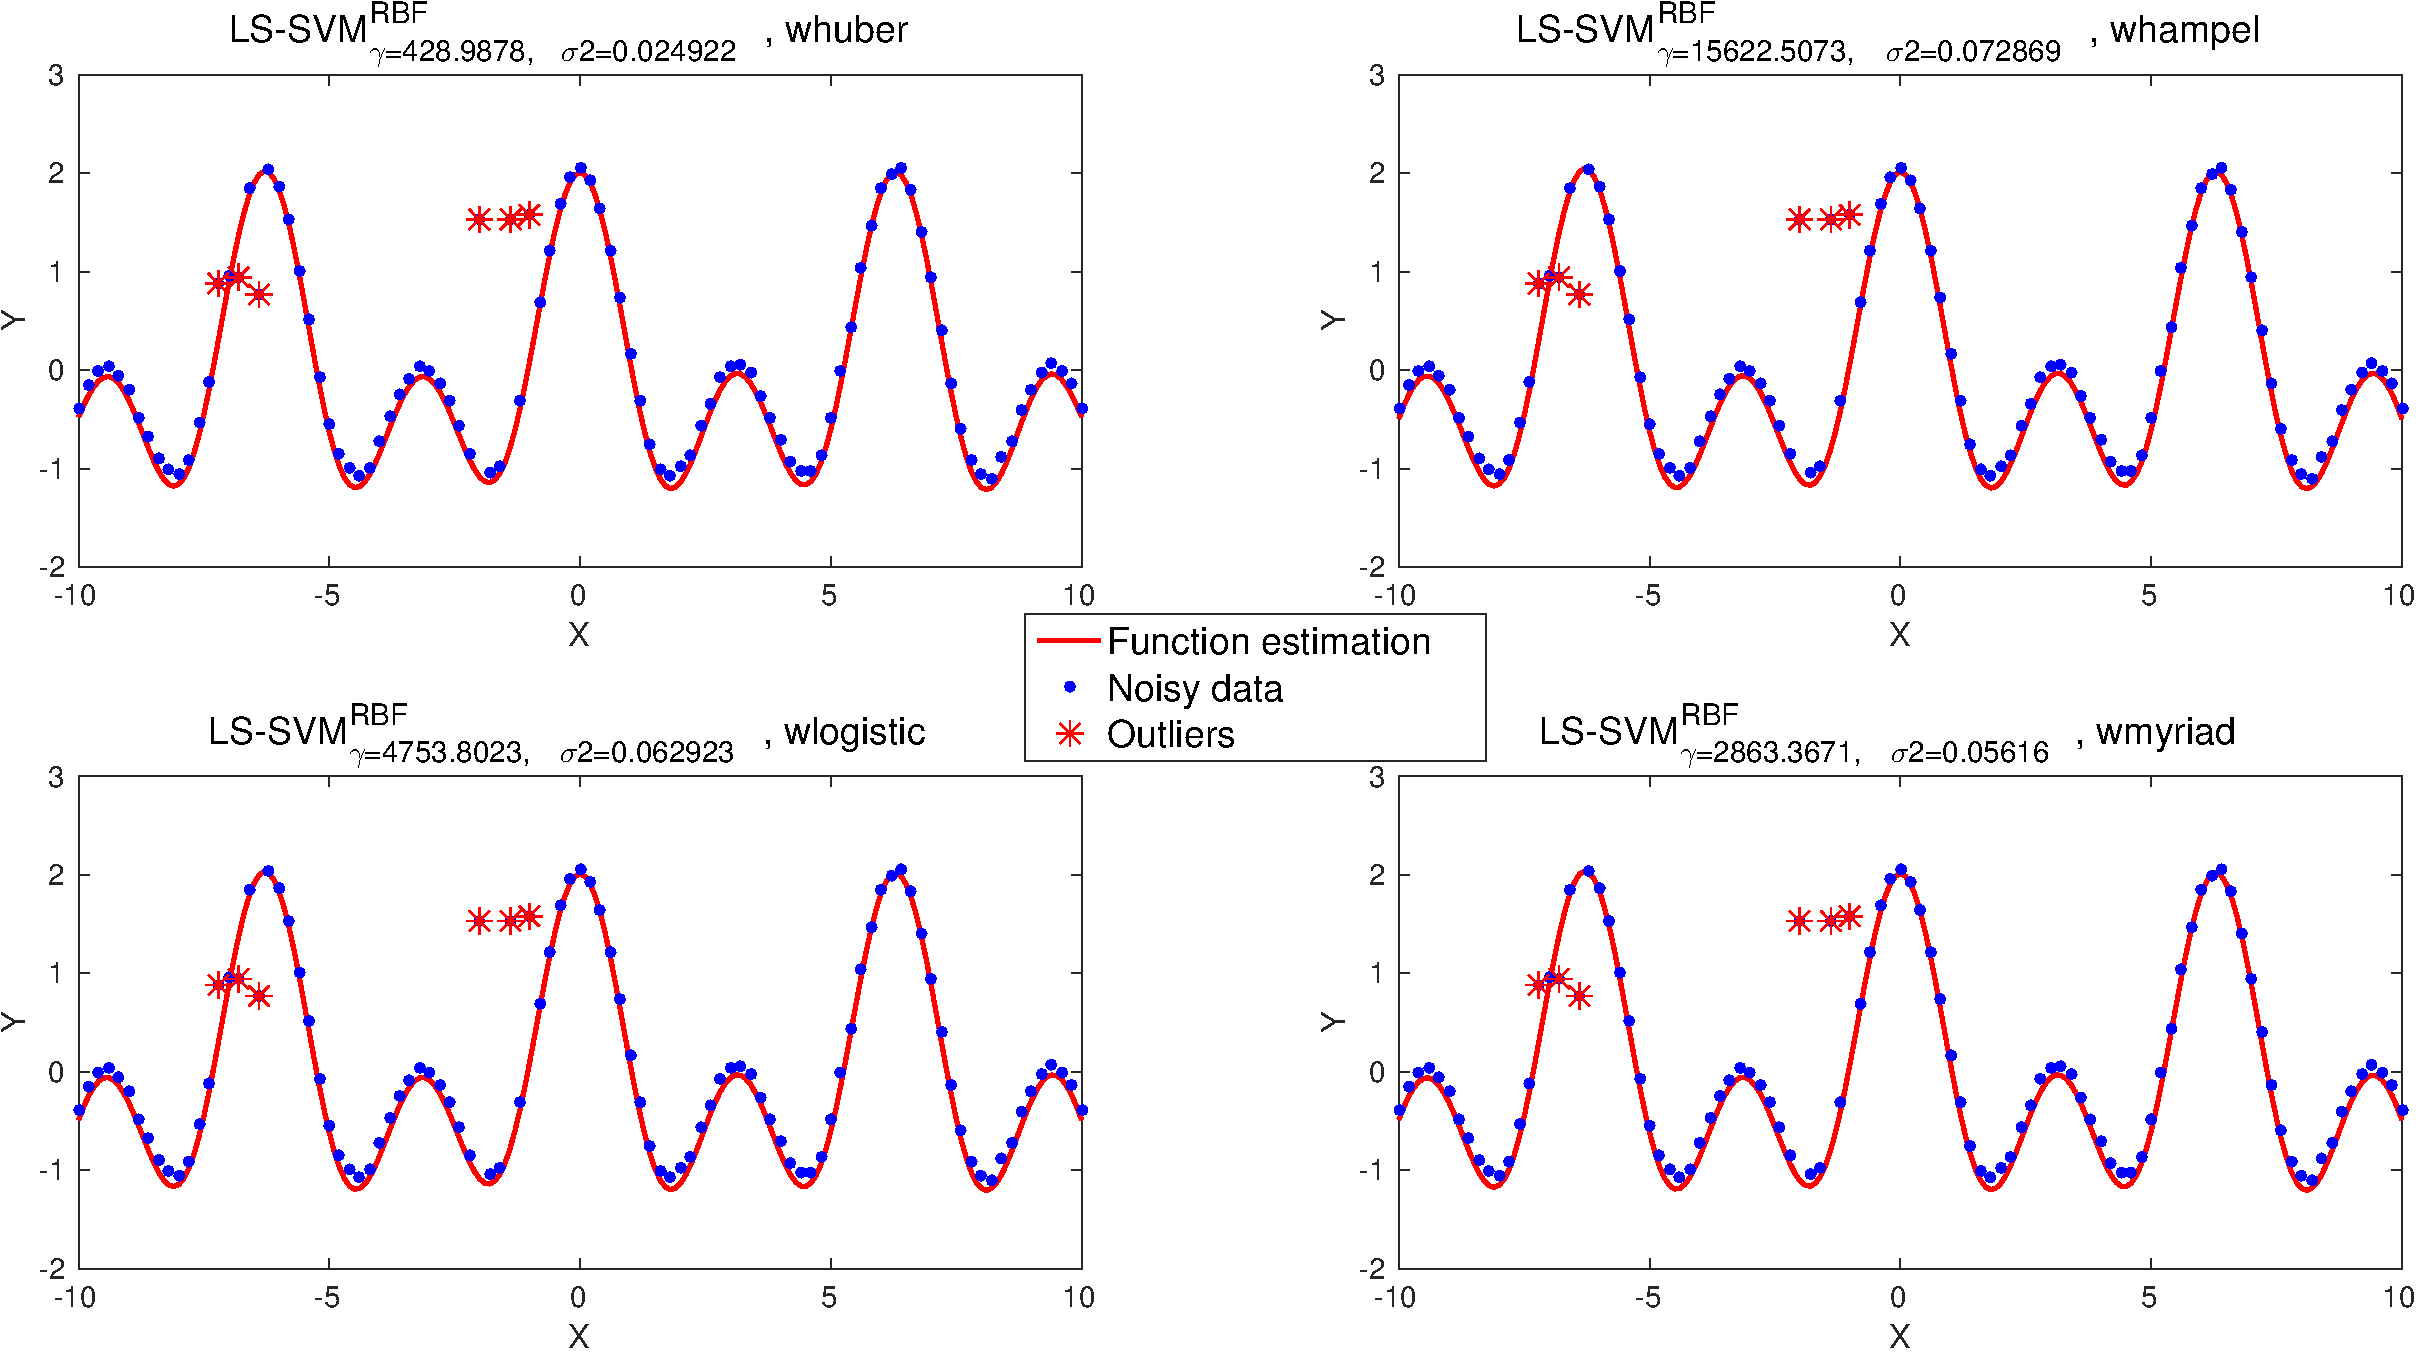
\includegraphics[scale=.40]{bayes_robust.pdf}
    \caption{Bayesian robust function estimation}
    \label{fig:bayes_robust}
\end{figure}

\newpage
The mean absolute error (MAE) is prefered over the classical mean
squared error (MSE) because of its ability to deal with outliers
better. Indeed, the MAE gives less importance to the points that are
further away from the mean than MSE.

\section{Applications: Santa-Fe dataset}

The dataset we work with in this last section represents a time serie
collected from an experiment with a laser
\footnote{http://www-psych.stanford.edu/~andreas/Time-Series/SantaFe.html}). It
has been split into a training set and a test set, as illustrated on
figure \ref{fig:santa_fe}. The blue part, will be used to train our
model with the goal of predicting the red part.

\begin{figure}[H]
    \centering
    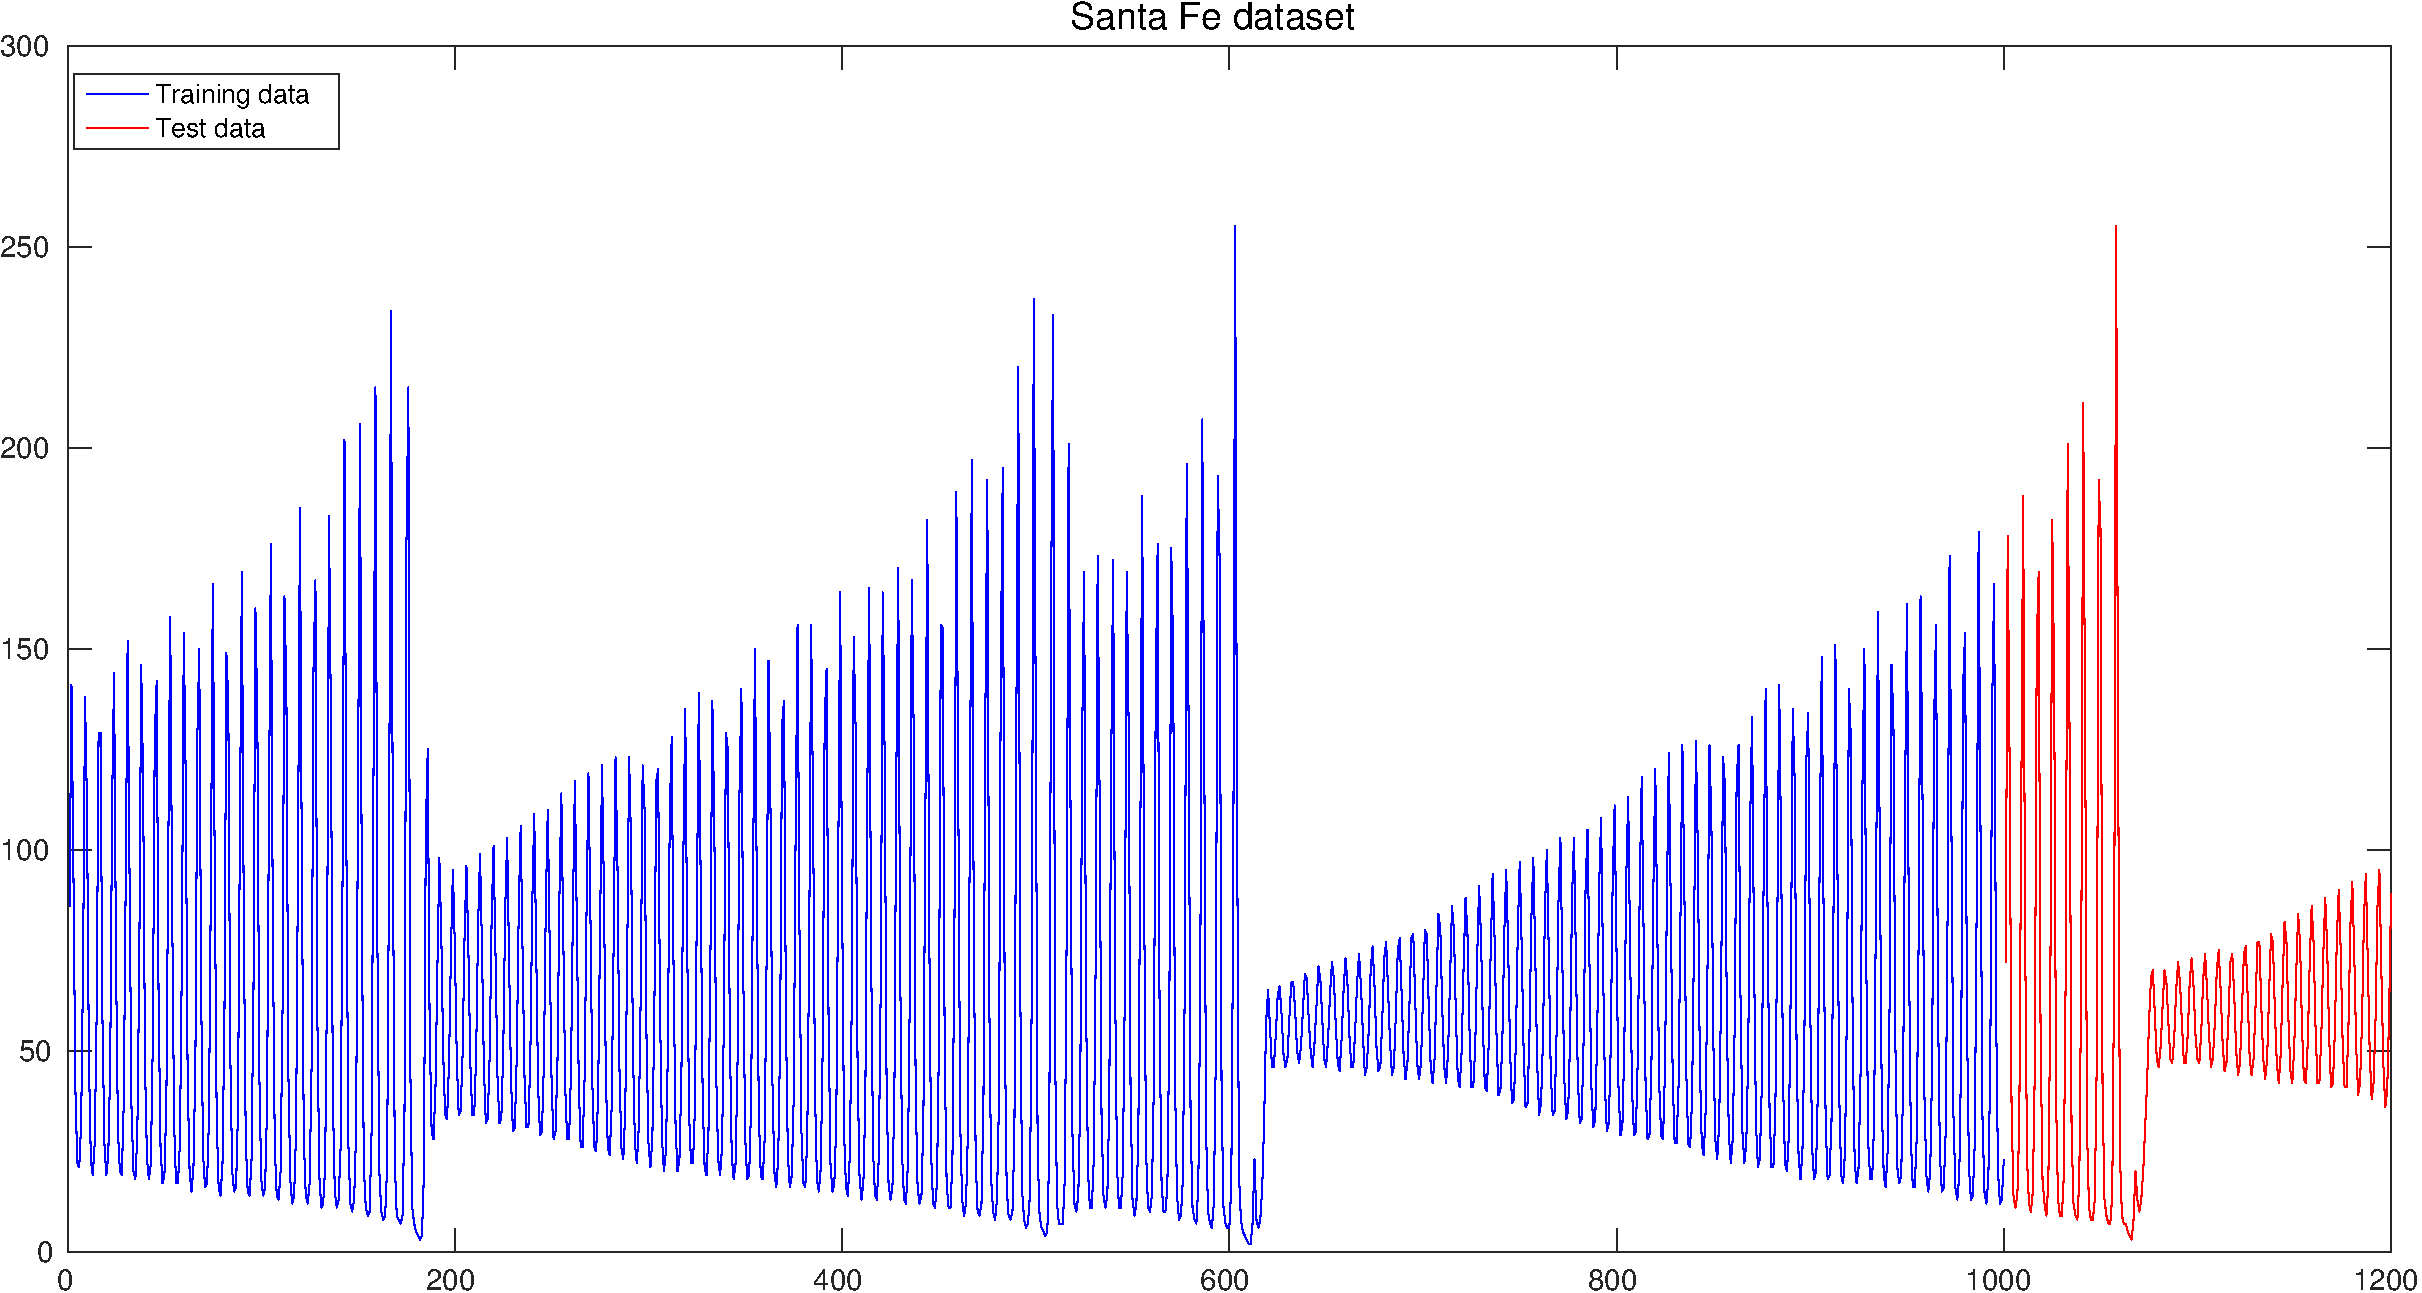
\includegraphics[scale=.40]{santafe_dataset.pdf}
    \caption{Time serie (santa fe dataset)}
    \label{fig:santa_fe}
\end{figure}

As suggested in the exercise, I optimized the kernel parameter
$\sigma^2$ and the hyperparameter $\gamma$ via the use of
\emph{tunelssvm} with crossvalidation on the training set. Then I
proceeded to determine what would be the best \emph{order} to use by
looking at the mean squared error between the predictions and the
actual value of the test set via a systematic model building over a
range of possible values (see figure \ref{fig:santa_prediction} for
results):

\begin{lstlisting}
mse_error = zeros(20,1); i = 1;
for order=5:5:100
    X=windowize(Z,1:(order+1));
    Y=X(:,end); X=X(:,1:order);

    [gam,sig2]=tunelssvm({X,Y,'f',[],[],'RBF_kernel'},'simplex','crossvalidatelssvm',{10,'mse'});
    [alpha,b]=trainlssvm({X,Y,'f',gam,sig2});

    horizon = length(Ztest)-order;
    Zpt = predict({X, Y, 'f', gam, sig2},Ztest(1:order), horizon);
    mse_error(i) = sqrt(mse(Zpt-Ztest(order+1:end)));
    i = i + 1;
end

% building best model based on order selection
order=60;
X=windowize(Z,1:(order+1));
Y=X(:,end); X=X(:,1:order);
[gam,sig2]=tunelssvm({X,Y,'f',[],[],'RBF_kernel'},'simplex','crossvalidatelssvm',{10,'mse'});
[alpha,b]=trainlssvm({X,Y,'f',gam,sig2});
horizon = length(Ztest)-order;
Zpt = predict({X, Y, 'f', gam, sig2},Ztest(1:order), horizon);
\end{lstlisting}

\begin{figure}[H]
    \centering
    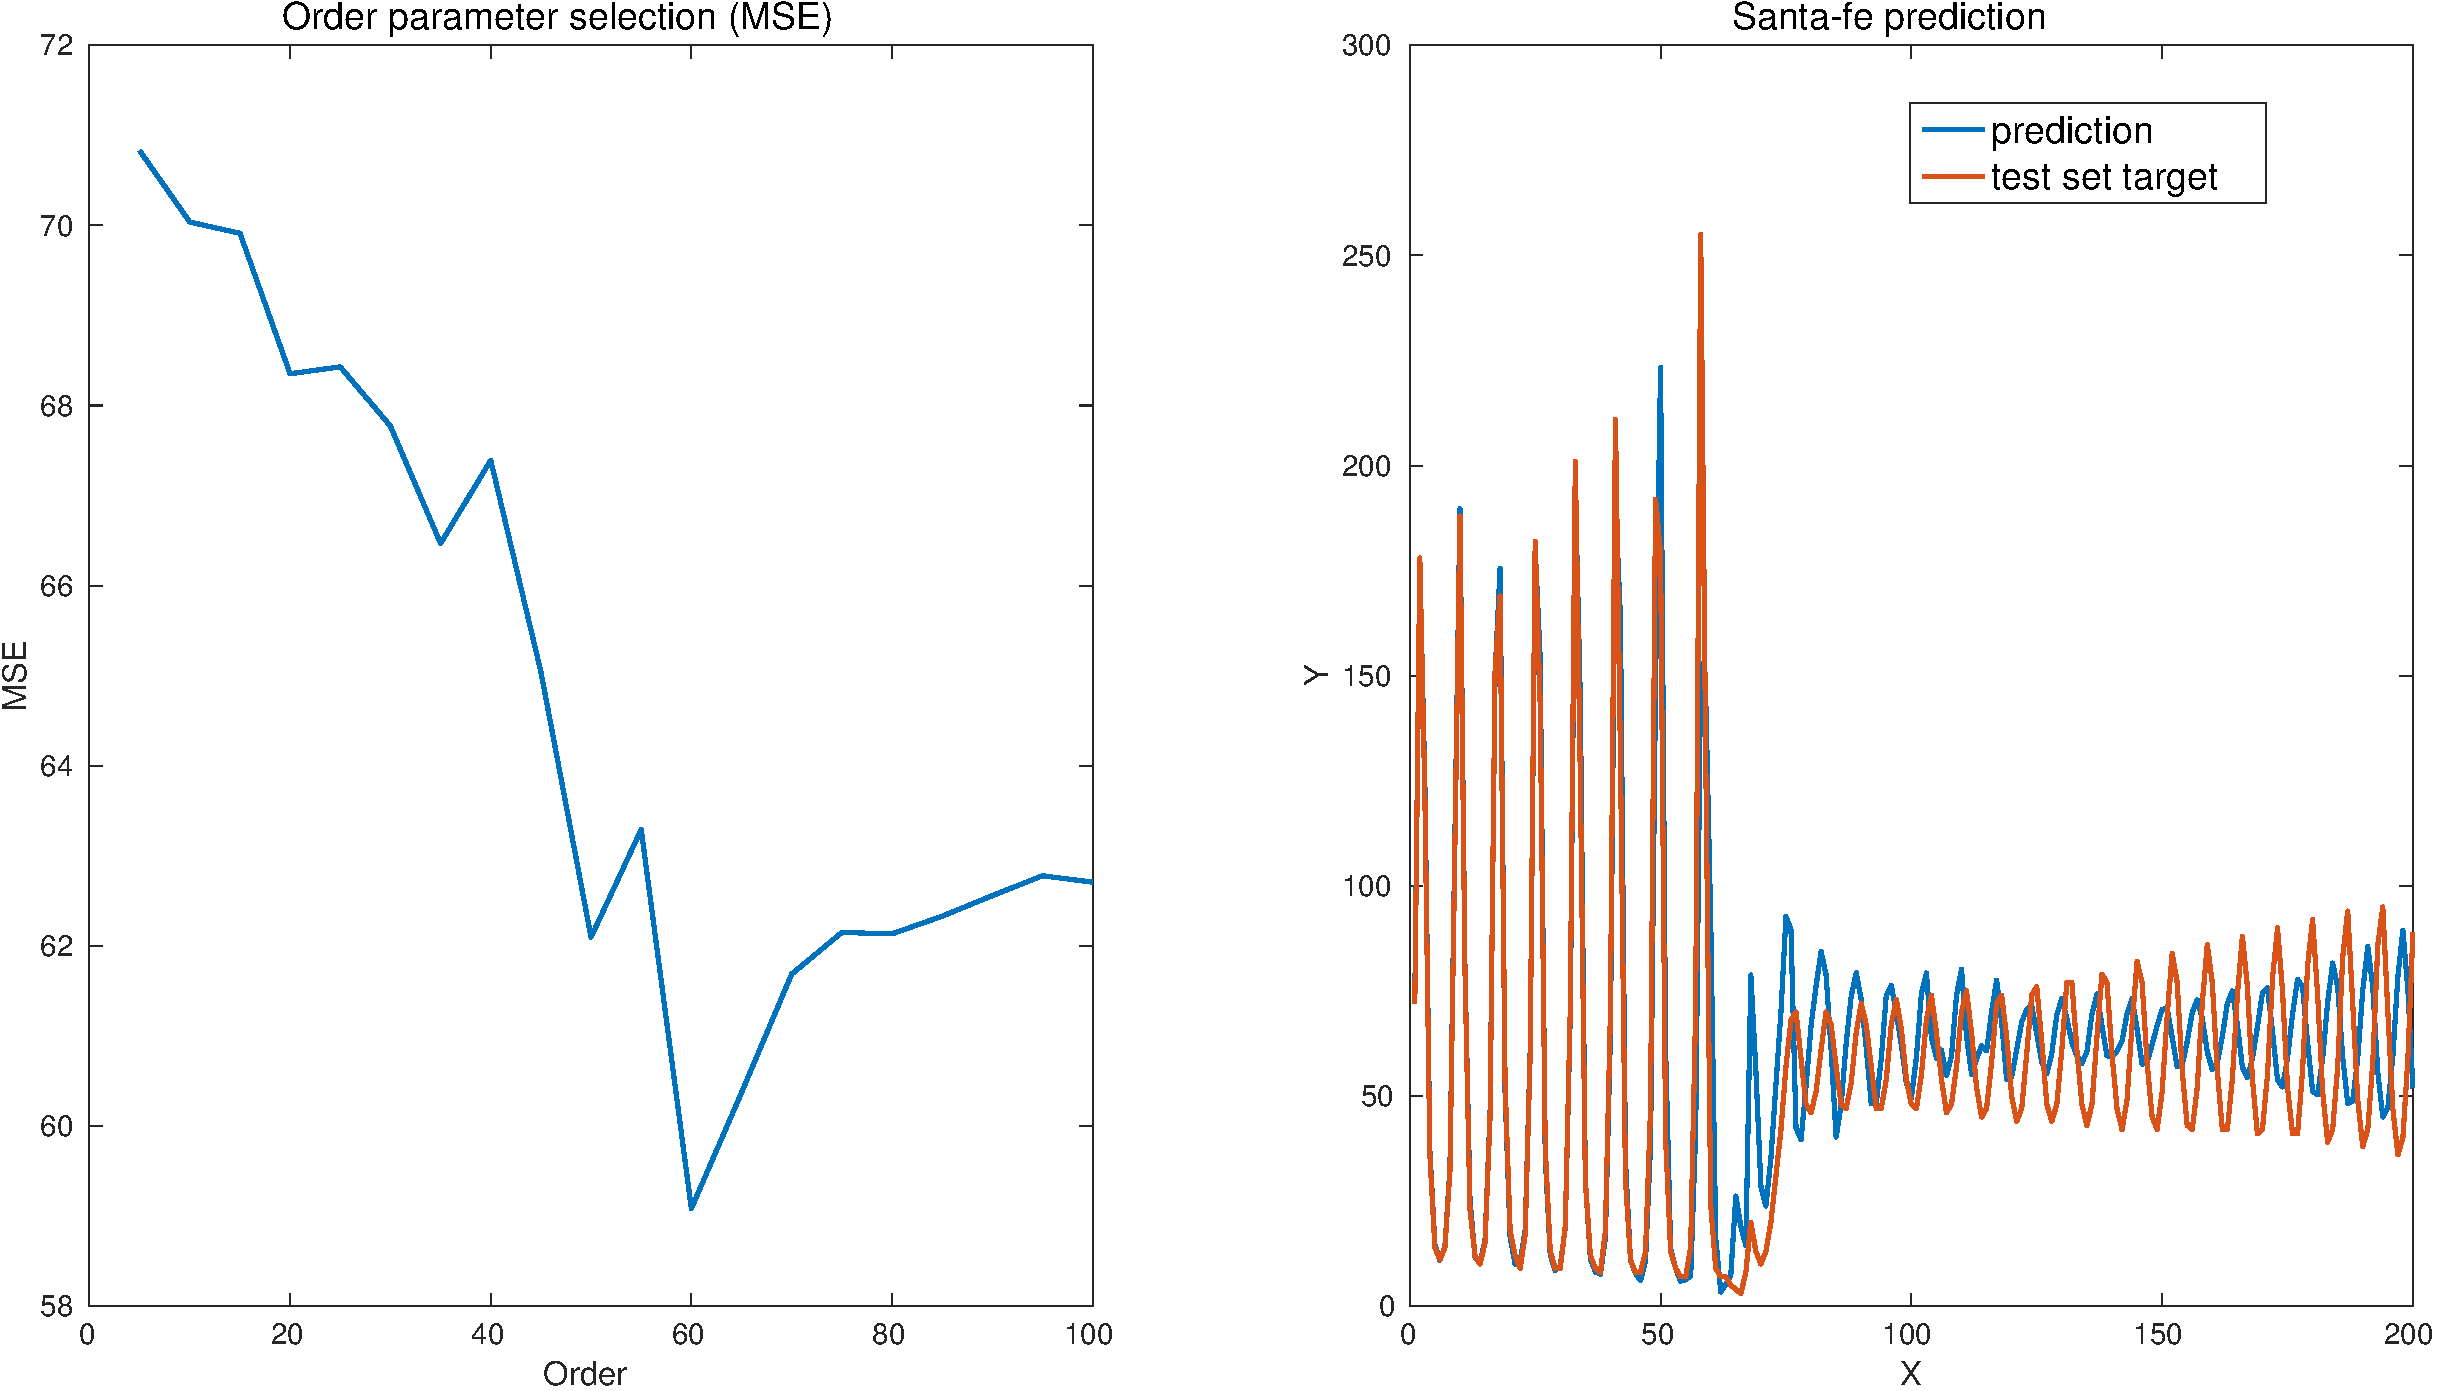
\includegraphics[scale=.40]{santafe_prediction.pdf}
    \caption{Left: MSE for different values of order, right: prediction}
    \label{fig:santa_prediction}
\end{figure}

In light of the previous results, it would seem that an order of 60
leads to better results than the suggested 50. However, one can wonder
whether it is possible to obtain even better prediction. For lack of
time, I did not investigate this further, but I will try to bring an
update for the examination.

\end{document}
